%% Copernicus Publications Manuscript Preparation Template for LaTeX Submissions
%DIF LATEXDIFF DIFFERENCE FILE
%DIF DEL 01-draft.tex    Sat Jun 11 14:31:29 2022
%DIF ADD 02-revise.tex   Sun Jun 12 08:54:37 2022
%% ---------------------------------
%% This template should be used for copernicus.cls
%% The class file and some style files are bundled in the Copernicus Latex Package, which can be downloaded from the different journal webpages.
%% For further assistance please contact Copernicus Publications at: production@copernicus.org
%% https://publications.copernicus.org/for_authors/manuscript_preparation.html

%% Please use the following documentclass and journal abbreviations for preprints and final revised papers.

%% 2-column papers and preprints
\documentclass[hess, manuscript]{copernicus}

%% Journal abbreviations (please use the same for preprints and final revised papers)
% Hydrology and Earth System Sciences (hess)

%% \usepackage commands included in the copernicus.cls:
%\usepackage[german, english]{babel}
%\usepackage{tabularx}
%\usepackage{cancel}
%\usepackage{multirow}
%\usepackage{supertabular}
%\usepackage{algorithmic}
%\usepackage{algorithm}
%DIF 24c24
%DIF < %\usepackage{amsthm}
%DIF -------
\usepackage{amsthm}   % use mathematics %DIF > 
%DIF -------
%\usepackage{float}
%\usepackage{subfig}
%\usepackage{rotating}
\usepackage{textcomp} % use %
%DIF 29a29-35
 %DIF > 
\newcommand\todo[1]{\textcolor{red}{! #1.}} %DIF > 
\usepackage{booktabs} % use tables %DIF > 
 %DIF > 
\usepackage{xr-hyper} % use cross references in two tex files %DIF > 
\externaldocument{materials} % link the external document %DIF > 
 %DIF > 
%DIF -------
\usepackage{hyperref} % use hyperlinks
%DIF < \hypersetup{colorlinks=true, citecolor=blue}
%DIF -------
\hypersetup{colorlinks=true, citecolor=blue, linkcolor=blue, urlcolor=blue} %DIF > 
%DIF PREAMBLE EXTENSION ADDED BY LATEXDIFF
%DIF UNDERLINE PREAMBLE %DIF PREAMBLE
\RequirePackage[normalem]{ulem} %DIF PREAMBLE
\RequirePackage{color}\definecolor{RED}{rgb}{1,0,0}\definecolor{BLUE}{rgb}{0,0,1} %DIF PREAMBLE
\providecommand{\DIFaddtex}[1]{{\protect\color{blue}\uwave{#1}}} %DIF PREAMBLE
\providecommand{\DIFdeltex}[1]{{\protect\color{red}\sout{#1}}}                      %DIF PREAMBLE
%DIF SAFE PREAMBLE %DIF PREAMBLE
\providecommand{\DIFaddbegin}{} %DIF PREAMBLE
\providecommand{\DIFaddend}{} %DIF PREAMBLE
\providecommand{\DIFdelbegin}{} %DIF PREAMBLE
\providecommand{\DIFdelend}{} %DIF PREAMBLE
\providecommand{\DIFmodbegin}{} %DIF PREAMBLE
\providecommand{\DIFmodend}{} %DIF PREAMBLE
%DIF FLOATSAFE PREAMBLE %DIF PREAMBLE
\providecommand{\DIFaddFL}[1]{\DIFadd{#1}} %DIF PREAMBLE
\providecommand{\DIFdelFL}[1]{\DIFdel{#1}} %DIF PREAMBLE
\providecommand{\DIFaddbeginFL}{} %DIF PREAMBLE
\providecommand{\DIFaddendFL}{} %DIF PREAMBLE
\providecommand{\DIFdelbeginFL}{} %DIF PREAMBLE
\providecommand{\DIFdelendFL}{} %DIF PREAMBLE
%DIF HYPERREF PREAMBLE %DIF PREAMBLE
\providecommand{\DIFadd}[1]{\texorpdfstring{\DIFaddtex{#1}}{#1}} %DIF PREAMBLE
\providecommand{\DIFdel}[1]{\texorpdfstring{\DIFdeltex{#1}}{}} %DIF PREAMBLE
%DIF LISTINGS PREAMBLE %DIF PREAMBLE
\RequirePackage{listings} %DIF PREAMBLE
\RequirePackage{color} %DIF PREAMBLE
\lstdefinelanguage{DIFcode}{ %DIF PREAMBLE
%DIF DIFCODE_UNDERLINE %DIF PREAMBLE
  moredelim=[il][\color{red}\sout]{\%DIF\ <\ }, %DIF PREAMBLE
  moredelim=[il][\color{blue}\uwave]{\%DIF\ >\ } %DIF PREAMBLE
} %DIF PREAMBLE
\lstdefinestyle{DIFverbatimstyle}{ %DIF PREAMBLE
	language=DIFcode, %DIF PREAMBLE
	basicstyle=\ttfamily, %DIF PREAMBLE
	columns=fullflexible, %DIF PREAMBLE
	keepspaces=true %DIF PREAMBLE
} %DIF PREAMBLE
\lstnewenvironment{DIFverbatim}{\lstset{style=DIFverbatimstyle}}{} %DIF PREAMBLE
\lstnewenvironment{DIFverbatim*}{\lstset{style=DIFverbatimstyle,showspaces=true}}{} %DIF PREAMBLE
%DIF END PREAMBLE EXTENSION ADDED BY LATEXDIFF

\begin{document}
\DIFdelbegin %DIFDELCMD < 

%DIFDELCMD < %%%
\DIFdelend %DIF > %%%%%%%%%%%%%%%%%%%%%%%%%%%%%%%%%%%%%%%%%%%%%%
%DIF > %%%%%%%%%%% Title and author %%%%%%%%%%%%%%%%%
%DIF > %%%%%%%%%%%%%%%%%%%%%%%%%%%%%%%%%%%%%%%%%%%%%%
\title{Climate and Cryosphere Cause \DIFaddbegin \DIFadd{Water Yield }\DIFaddend Regime Shifts in \DIFdelbegin \DIFdel{Water Yield over }\DIFdelend the  Upper Brahmaputra River \DIFaddbegin \DIFadd{basin}\DIFaddend }
\DIFdelbegin %DIFDELCMD < 

%DIFDELCMD < %%%
\DIFdelend % \Author[affil]{given_name}{surname}
\DIFdelbegin %DIFDELCMD < \Author[1]{Hao}{Li}
%DIFDELCMD < \Author[2]{Liu}{Liu}
%DIFDELCMD < \Author[3]{Baoying}{Shan}
%DIFDELCMD < %%%
\DIFdelend \DIFaddbegin \Author[1,2]{Hao}{Li}
\Author[3,2]{Baoying}{Shan}
\Author[1]{Liu}{Liu}
\DIFaddend \Author[4]{Lei}{Wang}
\DIFdelbegin %DIFDELCMD < \Author[1]{Akash}{Koppa}
%DIFDELCMD < \Author[5]{Feng}{Zhong}
%DIFDELCMD < %%%
\DIFdelend \DIFaddbegin \Author[2]{Akash}{Koppa}
\Author[5,2]{Feng}{Zhong}
\DIFaddend \Author[6]{Dongfeng}{Li}
\DIFdelbegin %DIFDELCMD < \Author[2]{Xuanxuan}{Wang}
%DIFDELCMD < \Author[2]{Wenfeng}{Liu}
%DIFDELCMD < %%%
\DIFdelend \DIFaddbegin \Author[1]{Xuanxuan}{Wang}
\Author[1]{Wenfeng}{Liu}
\Author[4]{Xiuping}{Li}
\DIFaddend \Author[7]{Zongxue}{Xu}

\DIFdelbegin %DIFDELCMD < \affil[1]{Hydro-Climate Extremes Lab, Ghent University, Ghent, Belgium}
%DIFDELCMD < \affil[2]{Center for Agricultural Water Research in China, China Agricultural University, Beijing, China}
%DIFDELCMD < %%%
\DIFdelend \DIFaddbegin \affil[1]{Center for Agricultural Water Research in China, China Agricultural University, Beijing, China}
\affil[2]{Hydro-Climate Extremes Lab, Ghent University, Ghent, Belgium}
\DIFaddend \affil[3]{Research Unit Knowledge-based Systems, Ghent University, Ghent, Belgium}
\affil[4]{Institute of Tibetan Plateau Research, Chinese Academy of China, Beijing, China}
\affil[5]{College of Hydrology and Water Resources, Hohai University, Nanjing, China}
\affil[6]{Department of Geography, National University of Singapore, Singapore}
\affil[7]{College of Water Sciences, Beijing Normal University, Beijing, China}

%% The [] brackets identify the author with the corresponding affiliation. 1, 2, 3, etc. should be inserted.
%% If an author is deceased, please mark the respective author name(s) with a dagger, e.g. "\Author[2,$\dag$]{Anton}{Smith}", and add a further "\affil[$\dag$]{deceased, 1 July 2019}".
%% If authors contributed equally, please mark the respective author names with an asterisk, e.g. "\Author[2,*]{Anton}{Smith}" and "\Author[3,*]{Bradley}{Miller}" and add a further affiliation: "\affil[*]{These authors contributed equally to this work.}".

\DIFdelbegin %DIFDELCMD < \correspondence{Liu Liu (liuliu@cau.edu.cn)}
%DIFDELCMD < %%%
\DIFdelend \DIFaddbegin \correspondence{Liu Liu (\url{liuliu@cau.edu.cn})}
\DIFaddend 

% These dates will be inserted by Copernicus Publications during the typesetting process.
\runningtitle{TEXT}
\runningauthor{TEXT}

\received{}
\pubdiscuss{} %% only important for two-stage journals
\revised{}
\accepted{}
\published{}
\firstpage{1}

\maketitle
%DIF > % Notes:
%DIF > %%  Simple present tense in the main text

%DIF > %%%%%%%%%%%%%%%%%%%%%%%%%%%%%%%%%%%%%%%%%%%%%%
%DIF > %%%%%%%%%%%%%%%% Abstract %%%%%%%%%%%%%%%%%%%%
%DIF > %%%%%%%%%%%%%%%%%%%%%%%%%%%%%%%%%%%%%%%%%%%%%%
\begin{abstract}
    Although evidence of hydrological responses to climate is abundant, \DIFdelbegin \DIFdel{changes in }\DIFdelend \DIFaddbegin \DIFadd{the reliable assessments of }\DIFaddend water yield (WY) \DIFdelbegin \DIFdel{in mountainous regionsdue to climate change and intensified cryospheric melt remain unclear, mainly because of limited observations and large uncertainties in cryosphere-hydrological modeling. 
In this study, we used annual runoff observations and a high-resolution precipitation dataset to examine the long-term changes in WY in }\DIFdelend \DIFaddbegin \DIFadd{over mountainous regions, such as }\DIFaddend the Upper Brahmaputra River (UBR) basin, \DIFdelbegin \DIFdel{as represented by six sub-basins from the stream head to downstream. 
    We found that WY generally increased }\DIFdelend \DIFaddbegin \DIFadd{remain unclear due to intensified cryospheric changes. 
    Based on multi-station runoff observations, we examine long-term WY changes }\DIFaddend during 1982--2013 \DIFdelbegin \DIFdel{, but regime shifts were detected }\DIFdelend \DIFaddbegin \DIFadd{in the  UBR basin, and find there are in general hydrological regime shifts }\DIFaddend in the late 1990s\DIFdelbegin \DIFdel{. Moreover, the direction of the changes in WY reversed from increasing to decreasing in recent years despite the magnitude of the changes continually increasing from less than }\DIFdelend \DIFaddbegin \DIFadd{; 
    magnitude increases in WY range from $\sim$}\DIFaddend 10\% to \DIFdelbegin \DIFdel{80.5\%. 
Furthermore, we used }\DIFdelend \DIFaddbegin \DIFadd{$\sim$80\%, while its directions reverse from upward to downward after the late 1990s.
    Then, }\DIFaddend the double mass curve \DIFdelbegin \DIFdel{technique }\DIFdelend \DIFaddbegin \DIFadd{(DMC) technique is used }\DIFaddend to assess the effects of climate, vegetation, and \DIFdelbegin \DIFdel{the }\DIFdelend cryosphere on WY \DIFdelbegin \DIFdel{. The results showed that the }\DIFdelend \DIFaddbegin \DIFadd{changes. 
    Results show that }\DIFaddend climate and cryosphere together \DIFdelbegin \DIFdel{contributed }\DIFdelend \DIFaddbegin \DIFadd{contribute }\DIFaddend to over 80\% of \DIFdelbegin \DIFdel{the magnitude increases in WY over }\DIFdelend \DIFaddbegin \DIFadd{magnitude increases of WY in }\DIFaddend the entire UBR basin\DIFdelbegin \DIFdel{. 
However, the combined effects were }\DIFdelend \DIFaddbegin \DIFadd{, in which the role of vegetation is nearly negligible.
    The combined effects, however, are }\DIFaddend either offsetting or additive, \DIFdelbegin \DIFdel{further }\DIFdelend leading to slight or substantial magnitude increases, respectively\DIFdelbegin \DIFdel{, in which the role of vegetation was nearly negligible. 
    Nevertheless, we found that meltwater from the cryosphere had the potential to alleviate the loss of water availability, which mainly resulted from reduced effective precipitation in most regions}\DIFdelend \DIFaddbegin \DIFadd{. 
    Climate change, particularly precipitation decrease leads to the downward WY trend in recent years,
    while melt waters under global warming may alleviate the water shortage in some basins}\DIFaddend . 
    Therefore, the combined effects of climate and cryosphere \DIFdelbegin \DIFdel{changes }\DIFdelend \DIFaddbegin \DIFadd{on WY }\DIFaddend should be considered in \DIFdelbegin \DIFdel{ecological restoration and }\DIFdelend \DIFaddbegin \DIFadd{future }\DIFaddend water resources management \DIFaddbegin \DIFadd{over mountainous basins}\DIFaddend , particularly involving co-benefits \DIFdelbegin \DIFdel{for }\DIFdelend \DIFaddbegin \DIFadd{between }\DIFaddend upstream and downstream regions.
\end{abstract}

\introduction
Water yield (WY) in \DIFdelbegin \DIFdel{mountains }\DIFdelend \DIFaddbegin \DIFadd{mountainous watersheds }\DIFaddend is crucial for sustaining fragile ecosystems in \DIFdelbegin \DIFdel{the }\DIFdelend headwaters, supplying valuable freshwater resources to downstream lowlands, and balancing co-benefits between \DIFdelbegin \DIFdel{the }\DIFdelend upstream and downstream areas, especially for large transboundary river systems \citep{viviroli2011climate}. 
In mountainous \DIFdelbegin \DIFdel{regions, changes in WY }\DIFdelend \DIFaddbegin \DIFadd{watersheds, WY changes }\DIFaddend have been commonly, but separately, attributed to climate \DIFdelbegin \DIFdel{changes }\DIFdelend \citep{dierauer2018climate,song2021river}, vegetation \citep{goulden2014mountain,zhou2021divergent}, and \DIFdelbegin \DIFdel{the cryosphere (such as glacial snow melt; see \mbox{%DIFAUXCMD
\citealt{kraaijenbrink2021climate}}\hspace{0pt}%DIFAUXCMD
).
These changes }\DIFdelend \DIFaddbegin \DIFadd{glaciers and snow melting \mbox{%DIFAUXCMD
\citep{huss2018global, biemans2019importance}}\hspace{0pt}%DIFAUXCMD
.
These }\DIFaddend are expected to alter the spatial and temporal distribution of water resources \citep{tang2019streamflow} and further threaten \DIFdelbegin \DIFdel{the }\DIFdelend water supply and food security downstream \citep{biemans2019importance}.
\DIFdelbegin \DIFdel{Despite some in situ observations and runoff estimates from state-of-the-art remote sensing technology, the total river runoff for the Third Pole}\DIFdelend \DIFaddbegin \DIFadd{The Qinghai-Tibet Plateau (QTP, see Figure \ref{fig:location}a)}\DIFaddend , which is also known as \DIFdelbegin \DIFdel{the }\DIFdelend “Asian Water Tower\DIFdelbegin \DIFdel{,}\DIFdelend ”\DIFdelbegin \DIFdel{has never been reliably quantified, and its responses to climate change remain unclear \mbox{%DIFAUXCMD
\citep{wang2021tp}}\hspace{0pt}%DIFAUXCMD
. 
Therefore, comprehensively assessing the impacts of the climate, vegetation, and cryosphere on long-term changes, particularly in magnitude and direction, in WY in this region is of great importance for the sustainable development of water resources and ecological environment \mbox{%DIFAUXCMD
\citep{yao2019recent}}\hspace{0pt}%DIFAUXCMD
. 
}%DIFDELCMD < 

%DIFDELCMD < %%%
\DIFdel{The Qinghai-Tibet Plateau (QTP), regarded as the center of the Third Pole, is one of the most sensitive and vulnerable mountainous regions to environmental changes \mbox{%DIFAUXCMD
\citep{kang2010review,yao2010glacial,yao2019recent} }\hspace{0pt}%DIFAUXCMD
and }\DIFdelend \DIFaddbegin \DIFadd{, }\DIFaddend supplies water resources for major rivers in Asia, such as Brahmaputra, Salween, Mekong, Yangtze, Yellow, and Indus Rivers \DIFdelbegin \DIFdel{. 
Changes in WY in this region are a crucial factor in }\DIFdelend \DIFaddbegin \DIFadd{\mbox{%DIFAUXCMD
\citep{kang2010review,yao2010glacial,yao2019recent}}\hspace{0pt}%DIFAUXCMD
. 
As such, WY changes over this region significantly affect }\DIFaddend the use of water resources, prevention of natural disasters, and protection of aquatic functions for the livelihoods of approximately two billion people \DIFdelbegin \DIFdel{in the area \mbox{%DIFAUXCMD
\citep{immerzeel2010climate}}\hspace{0pt}%DIFAUXCMD
. 
}\DIFdelend \DIFaddbegin \DIFadd{\mbox{%DIFAUXCMD
\citep{immerzeel2010climate}}\hspace{0pt}%DIFAUXCMD
. 
While, total river runoff has never been reliably assessed, and its responses to global warming remain unclear, despite some in-situ observations and runoff estimates from state-of-the-art remote sensing technology \mbox{%DIFAUXCMD
\citep{wang2021tp}}\hspace{0pt}%DIFAUXCMD
.
Therefore, comprehensively assessing the impacts of climate, vegetation, and cryosphere on long-term WY changes, particularly magnitude and direction, is of great importance for the sustainable development of water resources in the  QTP \mbox{%DIFAUXCMD
\citep{yao2019recent}}\hspace{0pt}%DIFAUXCMD
. 
}

\DIFaddend In recent years, changes in \DIFdelbegin \DIFdel{the }\DIFdelend climate, vegetation, and cryosphere have \DIFdelbegin \DIFdel{significantly affected the WY over the QTP\mbox{%DIFAUXCMD
\citep{bibi2018climatic}}\hspace{0pt}%DIFAUXCMD
}\DIFdelend \DIFaddbegin \DIFadd{affected WY in the QTP}\DIFaddend . 
For example, \citet{fan2015temperature} highlighted the \DIFdelbegin \DIFdel{effects of precipitation on the direction of change in WY over }\DIFdelend \DIFaddbegin \DIFadd{important role of precipitation in WY increases in }\DIFaddend the Salween and Mekong River basins. \citet{li2020substantial} \DIFdelbegin \DIFdel{determined }\DIFdelend \DIFaddbegin \DIFadd{found }\DIFaddend that elevated precipitation and \DIFdelbegin \DIFdel{warming-induced changes in glacial snow patterns }\DIFdelend \DIFaddbegin \DIFadd{cryosphere changes }\DIFaddend both contributed to \DIFdelbegin \DIFdel{the magnitude of the increase in WY for }\DIFdelend \DIFaddbegin \DIFadd{substantial WY increases in }\DIFaddend the Tuotuo River \DIFdelbegin \DIFdel{(a headwater of the Yangtze River)}\DIFdelend \DIFaddbegin \DIFadd{basin}\DIFaddend . Similarly, \citet{lutz2014consistent} projected that increased precipitation near the Salween and Mekong Rivers and accelerated meltwater near the Indus River caused \DIFdelbegin \DIFdel{major changes  in WY . 
Moreover, the role of vegetation in mountain water resourcesis important. }\DIFdelend \DIFaddbegin \DIFadd{significant WY changes. 
Vegetation has also been proven to be vital for mountainous water resources; }\DIFaddend \citet{li2017grassland} showed that \DIFdelbegin \DIFdel{increased evapotranspiration}\DIFdelend \DIFaddbegin \DIFadd{evaporation}\DIFaddend , mostly due to grassland restoration, decreased \DIFdelbegin \DIFdel{the }\DIFdelend WY in the Yangtze River basin, while \citet{li2021vegetation} suggested that vegetation greening \DIFdelbegin \DIFdel{was mainly linked to the positive WY trend }\DIFdelend \DIFaddbegin \DIFadd{may change the seasonality of water resources and increase WY }\DIFaddend during the dry season \DIFdelbegin \DIFdel{over the Brahmaputra River}\DIFdelend \DIFaddbegin \DIFadd{in the UBR basin}\DIFaddend .

Although a growing body of evidence has shown that WY is affected by climate, vegetation, and cryosphere in the QTP, most studies \DIFdelbegin \DIFdel{have focused on individual sub-basins and have not considered }\DIFdelend \DIFaddbegin \DIFadd{focus on individual basins, and also do not consider }\DIFaddend these three aspects together\DIFdelbegin \DIFdel{throughout this large and understudied region \mbox{%DIFAUXCMD
\citep{dierauer2018climate, goulden2014mountain,kraaijenbrink2021climate, song2021river,zhou2021divergent}}\hspace{0pt}%DIFAUXCMD
. Therefore}\DIFdelend \DIFaddbegin \DIFadd{. As such}\DIFaddend , previous results may not fully reveal the spatial \DIFdelbegin \DIFdel{variability in the region}\DIFdelend \DIFaddbegin \DIFadd{variabilities in WY}\DIFaddend . 
Of specific interest is the Upper Brahmaputra River (UBR\DIFaddbegin \DIFadd{, see Figure \ref{fig:location}a}\DIFaddend ) basin, which covers an area of over 198,636 km$^2$ \DIFdelbegin \DIFdel{(Table S1) }\DIFdelend and has large gradients in elevation, climate, and vegetation \citep{li2019spatiotemporal}.
\DIFdelbegin \DIFdel{Therefore, providing }\DIFdelend \DIFaddbegin \DIFadd{Hence, it is imperative to provide }\DIFaddend a comprehensive, spatially differentiated study \DIFdelbegin \DIFdel{of the WY changes in the UBR basin that considers the joint effects of the }\DIFdelend \DIFaddbegin \DIFadd{considering the effects of }\DIFaddend climate, vegetation, and cryosphere \DIFdelbegin \DIFdel{is imperative}\DIFdelend \DIFaddbegin \DIFadd{on WY changes in this region}\DIFaddend . 
However, studies of WY changes in \DIFdelbegin \DIFdel{this region }\DIFdelend \DIFaddbegin \DIFadd{the UBR basin }\DIFaddend are significantly hindered by the sparse network of hydrological observation stations \citep{li2019spatiotemporal,wang2021tp,yao2019recent}, which leads to large uncertainties in \DIFdelbegin \DIFdel{WY forecastsand, thus}\DIFdelend \DIFaddbegin \DIFadd{river flow forecasts}\DIFaddend , \DIFaddbegin \DIFadd{and thus }\DIFaddend water resources assessments.
\DIFdelbegin \DIFdel{In addition}\DIFdelend \DIFaddbegin \DIFadd{Also}\DIFaddend , current precipitation estimates are highly uncertain owing to the complex topography of \DIFdelbegin \DIFdel{the }\DIFdelend \DIFaddbegin \DIFadd{this }\DIFaddend region, which limits the ability to accurately model the relationships between precipitation and runoff \citep{sun2020precipitation}. 
Lastly, the present \DIFdelbegin \DIFdel{limited understanding of WY responses to the joint interaction of the }\DIFdelend \DIFaddbegin \DIFadd{inadequate understanding of hydrological responses to complex interactions among }\DIFaddend climate, vegetation, and cryosphere \DIFdelbegin \DIFdel{has become the biggest challenge for developing accurate physically-based cryosphere-hydrological models \mbox{%DIFAUXCMD
\citep{pellicciotti2012challenges}}\hspace{0pt}%DIFAUXCMD
. Nevertheless}\DIFdelend \DIFaddbegin \DIFadd{limits the application of hydrological models in these mountainous watersheds \mbox{%DIFAUXCMD
\citep{pellicciotti2012challenges}}\hspace{0pt}%DIFAUXCMD
. 
While}\DIFaddend , long-term \DIFdelbegin \DIFdel{runoff data and }\DIFdelend \DIFaddbegin \DIFadd{observed runoff records and recent }\DIFaddend high-resolution \DIFdelbegin \DIFdel{satellite records of climate and vegetation cover provide a potential pathway for determining their relationships using statistical }\DIFdelend \DIFaddbegin \DIFadd{precipitation datasets give a pathway for using statistical methods to estimate runoff responses to warming in the UBR basin. 
}\DIFaddend 

\DIFdelbegin \DIFdel{In this study , we collected annual runoff data for 1982--2013 from six hydrological stations to }\DIFdelend \DIFaddbegin \DIFadd{Hence, this study here jointly assesses historical WY responses to climate warming and associated environmental changes in the UBR basin. To do this, we collect multi-station runoff observations and }\DIFaddend detect long-term \DIFdelbegin \DIFdel{changes in the WY over the }\DIFdelend \DIFaddbegin \DIFadd{WY changes during 1982--2013 in the }\DIFaddend UBR basin. \DIFdelbegin \DIFdel{In addition, a modified }\DIFdelend \DIFaddbegin \DIFadd{And then, we use the }\DIFaddend double mass curve (DMC) \DIFdelbegin \DIFdel{method was implemented to assess the influence }\DIFdelend \DIFaddbegin \DIFadd{to estimate the effects }\DIFaddend of climate, vegetation, and \DIFdelbegin \DIFdel{the cryosphere on WY. 
Accordingly, the main objectives of this study were to identify the }\DIFdelend \DIFaddbegin \DIFadd{cryosphere on }\DIFaddend magnitude and direction \DIFdelbegin \DIFdel{of }\DIFdelend changes in WY\DIFdelbegin \DIFdel{based on observed runoff data and quantify the contributions of the climate, vegetation, and cryosphere to these changes}\DIFdelend . This study \DIFdelbegin \DIFdel{can provide a reference for physical-based cryosphere-hydrological modeling and important }\DIFdelend \DIFaddbegin \DIFadd{is expected to provide essential }\DIFaddend information for water resources \DIFdelbegin \DIFdel{and ecosystem management over }\DIFdelend \DIFaddbegin \DIFadd{management in }\DIFaddend the UBR basin and other mountainous \DIFdelbegin \DIFdel{regions}\DIFdelend \DIFaddbegin \DIFadd{watersheds}\DIFaddend . 

\section{Data and Methods}
\DIFaddbegin 

\DIFaddend \subsection{Study area}
The Brahmaputra River (known as the Yarlung Zangbo River, or YZR, in China), a transboundary river in the southern QTP, originates in the Gyama Langdzom Glacier and flows across China, India, and Bangladesh, before emptying into the Indian Ocean. The UBR basin is located above the Nuxia hydrological station (Figure \DIFdelbegin \DIFdel{1a}\DIFdelend \DIFaddbegin \DIFadd{\ref{fig:location}a}\DIFaddend ), and its \DIFaddbegin \DIFadd{river }\DIFaddend flow has significant implications \DIFdelbegin \DIFdel{for the ecology of the source region and }\DIFdelend \DIFaddbegin \DIFadd{on }\DIFaddend freshwater resources of South Asia. 
Here, we \DIFdelbegin \DIFdel{divided }\DIFdelend \DIFaddbegin \DIFadd{divide }\DIFaddend the UBR basin into the headstream (HYZR), upstream (UYZR), midstream (MYZR), downstream (LYZR), Nianchu River (NCR), and Lhasa River (LSR) \DIFdelbegin \DIFdel{by }\DIFdelend \DIFaddbegin \DIFadd{basins by the locations of }\DIFaddend hydrological stations (\DIFdelbegin \DIFdel{Figure 1b and Table S1), and analyzed WY changes over these six sub-basins to reveal spatial differences}\DIFdelend \DIFaddbegin \DIFadd{Table \ref{tab: table 1} and Figure \ref{fig:location}b)}\DIFaddend .

The elevation gradient and the distance to the ocean in the UBR basin together contribute to a large spatial variability in \DIFdelbegin \DIFdel{the climate \mbox{%DIFAUXCMD
\citep{sang2016precipitation,wang2020integration,wang2021vanishing}}\hspace{0pt}%DIFAUXCMD
}\DIFdelend \DIFaddbegin \DIFadd{climate \mbox{%DIFAUXCMD
\citep{sang2016precipitation}}\hspace{0pt}%DIFAUXCMD
}\DIFaddend . 
The annual precipitation in the HYZR basin is less than 400 mm, while that in the  LYZR basin is nearly 1000 mm\DIFdelbegin \DIFdel{(Figure S1). Similarly}\DIFdelend \DIFaddbegin \DIFadd{, and similarly}\DIFaddend , the annual actual \DIFdelbegin \DIFdel{evapotranspiration (AET) }\DIFdelend \DIFaddbegin \DIFadd{evaporation }\DIFaddend increases gradually from upstream to downstream areas (Figure \DIFdelbegin \DIFdel{S1}\DIFdelend \DIFaddbegin \DIFadd{\ref{figS:climate means}a+b}\DIFaddend ).
Meanwhile, water and energy availability modulate \DIFdelbegin \DIFdel{the }\DIFdelend vegetation conditions \citep{li2019greening}; vegetation cover increases dramatically from the HYZR to the LYZR basin (Figure \DIFdelbegin \DIFdel{S1). Furthermore, glacial snow meltwater from the cryosphere due to warming conditions has substantially affected the hydrology of }\DIFdelend \DIFaddbegin \DIFadd{\ref{figS:climate means}c). Additionally, cryospheric meltwater due to atmospheric warming has substantially altered hydrology conditions in }\DIFaddend this region \citep{cuo2019warming,yao2010glacial,wang2021tp}.

\DIFdelbegin %DIFDELCMD < \begin{figure*}[t]
%DIFDELCMD < 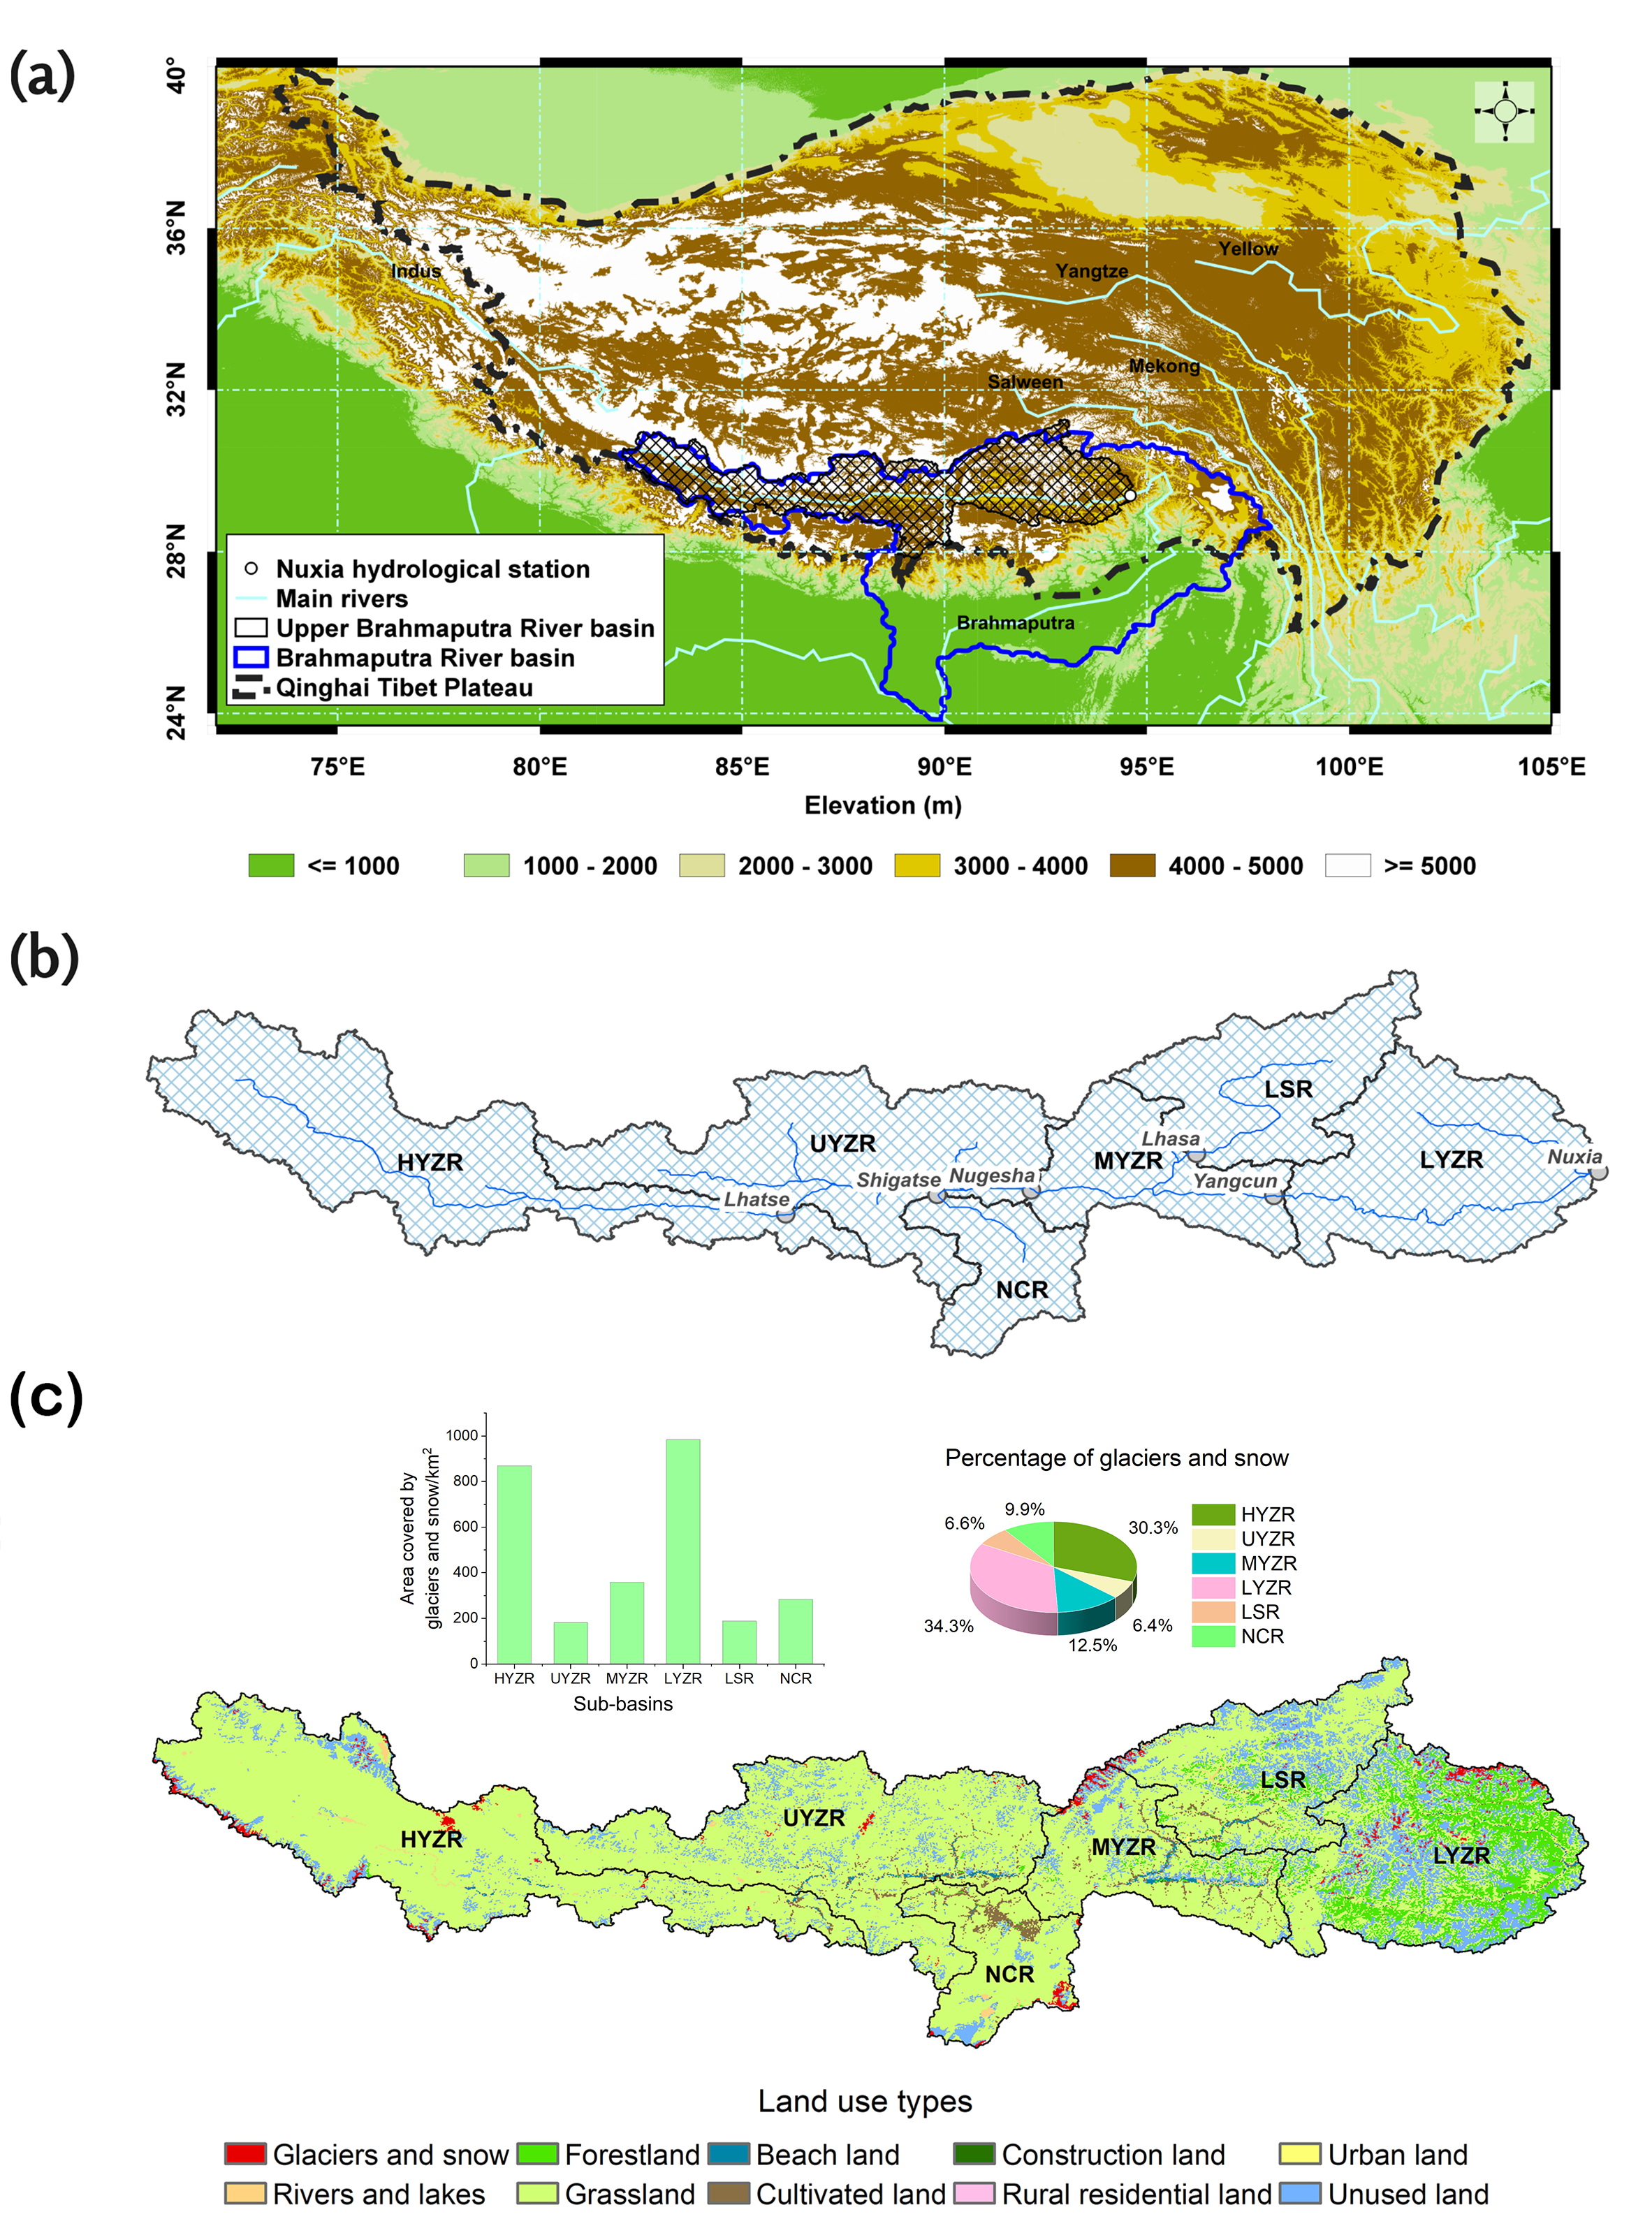
\includegraphics[width=12cm]{01-figures/Fig.1.png}
%DIFDELCMD < %%%
\DIFdelendFL \DIFaddbeginFL \begin{table}[hb]
    \centering
    \DIFaddendFL \caption{\DIFdelbeginFL \DIFdelFL{Location }\DIFdelendFL \DIFaddbeginFL \DIFaddFL{Information }\DIFaddendFL of \DIFdelbeginFL \DIFdelFL{(}\DIFdelendFL \DIFaddbeginFL \DIFaddFL{six basins divided by the locations of hydrological stations.   
    The column "TP" indicates the turning point using the Pettitt method, in which }\DIFaddendFL a \DIFdelbeginFL \DIFdelFL{) }\DIFdelendFL \DIFaddbeginFL \DIFaddFL{significant tuning point is labeled with *.
    Glaciers and snow area is acquired from }\DIFaddendFL the \DIFdelbeginFL \DIFdelFL{Upper Brahmaputra River }\DIFdelendFL \DIFaddbeginFL \DIFaddFL{land use and cover in 2000 }\DIFaddendFL (\DIFdelbeginFL \DIFdelFL{UBR}\DIFdelendFL \DIFaddbeginFL \DIFaddFL{see details in Dataset}\DIFaddendFL )\DIFdelbeginFL \DIFdelFL{basin over the Qinghai Tibet Plateau; (b}\DIFdelendFL \DIFaddbeginFL \DIFaddFL{.}}

    \begin{tabular}{ccccccc}
    \hline
    \DIFaddFL{Abbrevation }&
      \DIFaddFL{Full names }&
      \DIFaddFL{Station }&
      \begin{tabular}[c]{@{}c@{}}\DIFaddFL{Total }\\ \DIFaddFL{area (km$^2$}\DIFaddendFL )\DIFdelbeginFL \DIFdelFL{the six sub-basins delineated by
the }\DIFdelendFL \DIFaddbeginFL \end{tabular} &
      \begin{tabular}[c]{@{}c@{}}\DIFaddFL{Mean }\\ \DIFaddFL{elevation (m)}\end{tabular} &
      \begin{tabular}[c]{@{}c@{}}\DIFaddFL{Glaciers and snow }\\ \DIFaddFL{percentage (\%)}\end{tabular} &
      \begin{tabular}[c]{@{}c@{}}\DIFaddFL{TP}\end{tabular} \\ \hline
    \DIFaddFL{HYZR }& \DIFaddFL{Headstream    }& \DIFaddendFL Lhatse   \DIFaddbeginFL & \DIFaddFL{49}\DIFaddendFL ,\DIFaddbeginFL \DIFaddFL{739 }& \DIFaddFL{5061 }& \DIFaddFL{1.7  }& \DIFaddFL{1995  }\\
    \DIFaddFL{UYZR }& \DIFaddFL{Upstream      }& \DIFaddendFL Nugesha  \DIFaddbeginFL & \DIFaddFL{43}\DIFaddendFL ,\DIFaddbeginFL \DIFaddFL{916 }& \DIFaddFL{4985 }& \DIFaddFL{0.39 }& \DIFaddFL{1998* }\\
    \DIFaddFL{NCR  }& \DIFaddFL{Nianchu River }& \DIFaddendFL Shigatse \DIFaddbeginFL & \DIFaddFL{14}\DIFaddendFL ,\DIFaddbeginFL \DIFaddFL{359 }& \DIFaddFL{4733 }& \DIFaddFL{1.96 }& \DIFaddFL{1997* }\\
    \DIFaddFL{MYZR }& \DIFaddFL{Midstream     }& \DIFaddendFL Yangcun  \DIFaddbeginFL & \DIFaddFL{20}\DIFaddendFL ,\DIFaddbeginFL \DIFaddFL{004 }& \DIFaddFL{4681 }& \DIFaddFL{1.81 }& \DIFaddFL{1997* }\\
    \DIFaddFL{LSR  }& \DIFaddFL{Lhasa River   }& \DIFaddendFL Lhasa    \DIFaddbeginFL & \DIFaddFL{25}\DIFaddendFL ,\DIFdelbeginFL \DIFdelFL{and }\DIFdelendFL \DIFaddbeginFL \DIFaddFL{601 }& \DIFaddFL{4879 }& \DIFaddFL{0.72 }& \DIFaddFL{1996  }\\
    \DIFaddFL{LYZR }& \DIFaddFL{Downstream    }& \DIFaddendFL Nuxia    \DIFdelbeginFL \DIFdelFL{hydrological stations; and (c) the distribution of land use types and percentage
of area covered by glaciers and snow in 2015}\DIFdelendFL \DIFaddbeginFL & \DIFaddFL{45}\DIFaddendFL ,\DIFdelbeginFL \DIFdelFL{provided by National Tibetan Plateau Data Center.}%DIFDELCMD < \MBLOCKRIGHTBRACE
%DIFDELCMD < %%%
\DIFdelendFL \DIFaddbeginFL \DIFaddFL{017 }& \DIFaddFL{4586 }& \DIFaddFL{2.51 }& \DIFaddFL{1997  }\\ \hline
    \end{tabular}
    \label{tab: table 1}
\end{table}

\begin{figure*}[ht]
    \includegraphics[width=12cm]{02-figures/Figure1.png}
    \caption{\DIFaddFL{Location of (a) the Upper Brahmaputra River (UBR) basin in the Qinghai Tibet Plateau (QTP), which is from \mbox{%DIFAUXCMD
\citet{li2021vegetation}}\hspace{0pt}%DIFAUXCMD
, and (b) six basins divided by Lhatse, Nugesha, Shigatse, Yangcun, Lhasa, and Nuxia hydrological stations.}}
    \DIFaddendFL \label{fig:location}
\end{figure*}

\subsection{Dataset}
\DIFaddbegin \DIFadd{Here we collect annual runoff observations from 1982 to 2013 and convert the river flow ($m^{3}/s$) into runoff depth ($mm$). Also, we acquire high-resolution climate and vegetation data in the same time range, and further aggregate these gridded data into regional annual values by considering area-weighted effects (their temporal changes are shown in Figure \ref{figS:time series}).
}

\DIFaddend \subsubsection{Runoff data}
Annual runoff data between 1982 and 2013 \DIFaddbegin \DIFadd{used here come }\DIFaddend from six hydrological stations along the mainstream and major branches \DIFdelbegin \DIFdel{, which were provided by the Hydrology and Water Resources Survey Bureau of the Tibet Autonomous Region, were used in the study.
The }\DIFdelend \DIFaddbegin \DIFadd{in the UBR basin.
}\DIFaddend WY in the HYZR \DIFdelbegin \DIFdel{was determined by the runoff observed at the Lhatse hydrological }\DIFdelend \DIFaddbegin \DIFadd{is equal to runoff depth at Lhatse }\DIFaddend station, while \DIFdelbegin \DIFdel{the }\DIFdelend WY in other \DIFdelbegin \DIFdel{sub-basins was determined }\DIFdelend \DIFaddbegin \DIFadd{basins is calculated }\DIFaddend by the difference between runoff \DIFdelbegin \DIFdel{observed from gauging stations located at }\DIFdelend \DIFaddbegin \DIFadd{depth from }\DIFaddend the downstream station and that \DIFdelbegin \DIFdel{at }\DIFdelend \DIFaddbegin \DIFadd{from }\DIFaddend the upstream and branch stations. 
For example, WY in the MYZR basin \DIFdelbegin \DIFdel{was }\DIFdelend \DIFaddbegin \DIFadd{is }\DIFaddend equal to the difference between \DIFdelbegin \DIFdel{the observed annual runoff in the Yangcun hydrological }\DIFdelend \DIFaddbegin \DIFadd{runoff depth in Yangcun }\DIFaddend station and that in \DIFdelbegin \DIFdel{the }\DIFdelend Lhasa and Nugesha stations (Figure \DIFdelbegin \DIFdel{1b}\DIFdelend \DIFaddbegin \DIFadd{\ref{fig:location}b}\DIFaddend ).

\subsubsection{Climate data}
The most recent \DIFdelbegin \DIFdel{10 }\DIFdelend \DIFaddbegin \DIFadd{10x10 }\DIFaddend km gridded daily precipitation \DIFdelbegin \DIFdel{dataset was obtained from \mbox{%DIFAUXCMD
\citet{sun2020precipitation}}\hspace{0pt}%DIFAUXCMD
, which combined }\DIFdelend \DIFaddbegin \DIFadd{data, combining }\DIFaddend topographic and linear correction approaches based on 262 rain-gauge observations, \DIFdelbegin \DIFdel{and was applied }\DIFdelend \DIFaddbegin \DIFadd{is developed for the UBR basin by \mbox{%DIFAUXCMD
\citet{sun2020precipitation} }\hspace{0pt}%DIFAUXCMD
and here used }\DIFaddend to estimate regional annual precipitation (P)\DIFdelbegin \DIFdel{in this study.
Regional annual AETwas acquired from the }\DIFdelend \DIFaddbegin \DIFadd{. 
The maximum 2 m air temperature is obtained from China Meteorological Forcing Dataset \mbox{%DIFAUXCMD
\citep{he2020first}}\hspace{0pt}%DIFAUXCMD
.
Regional actual evaporation (AET) with a 0.25$^{\circ}$ spatial resolution is acquired from }\DIFaddend Global Land Evaporation Amsterdam Model (GLEAM) \DIFdelbegin \DIFdel{products with a spatial resolution of 0.25° 
}\DIFdelend \citep{martens2017gleam}. The \DIFdelbegin \DIFdel{effective precipitation (eP) was regarded as a proxy for climate in this study and was calculated as the difference between P and AET, as shown in Section 2.3.2}\DIFdelend \DIFaddbegin \DIFadd{evaporation product has been validated in different biome types in China and shown high correlations with in-situ eddy covariance AET \mbox{%DIFAUXCMD
\citep{yang2017multi}}\hspace{0pt}%DIFAUXCMD
}\DIFaddend .

\subsubsection{Vegetation data}
The leaf area index (LAI) \DIFdelbegin \DIFdel{data }\DIFdelend used in this study \DIFdelbegin \DIFdel{were obtained from the }\DIFdelend \DIFaddbegin \DIFadd{is obtained from }\DIFaddend Global Inventory Monitoring and Modelling System (GIMMS) \DIFdelbegin \DIFdel{, and spanned 1982 to 2015 }\DIFdelend \DIFaddbegin \DIFadd{LAI3g }\DIFaddend with a spatial resolution of 8\DIFdelbegin \DIFdel{km }\DIFdelend ×8 km \DIFdelbegin \DIFdel{. GIMMS LAI3g \mbox{%DIFAUXCMD
\citep{zhu2013global}}\hspace{0pt}%DIFAUXCMD
was }\DIFdelend \DIFaddbegin \DIFadd{\mbox{%DIFAUXCMD
\citep{zhu2013global}}\hspace{0pt}%DIFAUXCMD
. 
The product is }\DIFaddend generated using an artificial neural network trained on the Collection Terra Moderate Resolution Imaging Spectroradiometer (MODIS) LAI product and the latest version of GIMMS NDVI3g \DIFdelbegin \DIFdel{(normalized difference vegetation index) }\DIFdelend data for the same period, 
which has been proven to have an improved multi-sensor record harmonization scheme compared to other global LAI products \citep{forzieri2020increased,gonsamo2021greening}. 
\DIFdelbegin \DIFdel{Note that all gridded data were aggregated to regional values over each sub-basin on an annual time scale from 1982 to 2013, considering area-weighted effects. }\DIFdelend \DIFaddbegin 

\subsubsection{\DIFadd{Land use and cover}}
\DIFadd{The land use and cover in 2000 with a spatial resolution of 1x1 km is used to represent the land cover types in the UBR basin. The data is acquired from Resource and Environmental Science Data Center, and is here divided into seven primary land use types, including cultivated land, forestland, grassland, water body, urban land, unused land, and glaciers and snow (Figure \ref{figS:lucc}). %DIF > The data is developed by the land-use dynamic regionalization method based on land survey data and LANDSAT TM/ETM remote sensing images \citep{liu2014spatiotemporal}.
}\DIFaddend 

\subsection{Methodology}
\subsubsection{Trend and abruption analysis}
In this study, we \DIFdelbegin \DIFdel{used }\DIFdelend \DIFaddbegin \DIFadd{use }\DIFaddend the non-parametric Mann--Kendall test \citep{kendall1938new,mann1945nonparametric} to identify the \DIFdelbegin \DIFdel{trends }\DIFdelend \DIFaddbegin \DIFadd{trend }\DIFaddend in WY, and \DIFdelbegin \DIFdel{the non-parametric }\DIFdelend Pettitt abrupt detection \DIFdelbegin \DIFdel{method }\DIFdelend \citep{pettitt1979non} to identify the turning \DIFdelbegin \DIFdel{points }\DIFdelend \DIFaddbegin \DIFadd{point }\DIFaddend (TP) in WY\DIFdelbegin \DIFdel{. The }\DIFdelend \DIFaddbegin \DIFadd{, where the }\DIFaddend level of significance \DIFdelbegin \DIFdel{was }\DIFdelend \DIFaddbegin \DIFadd{is }\DIFaddend set at 0.05. 
We \DIFdelbegin \DIFdel{compared the average }\DIFdelend \DIFaddbegin \DIFadd{then compare the averages of }\DIFaddend WY before and after \DIFdelbegin \DIFdel{each }\DIFdelend \DIFaddbegin \DIFadd{the }\DIFaddend TP to reflect the magnitude \DIFdelbegin \DIFdel{of WY }\DIFdelend changes, and \DIFdelbegin \DIFdel{compared the trends before and after each TP }\DIFdelend \DIFaddbegin \DIFadd{compare the trends in two periods }\DIFaddend to reflect the direction \DIFdelbegin \DIFdel{of the }\DIFdelend changes.

\subsubsection{Double mass curve \DIFaddbegin \DIFadd{technique}\DIFaddend }
\DIFdelbegin \DIFdel{In a }\DIFdelend \DIFaddbegin \DIFadd{The DMC used here is a plot of the cumulative data of one variable versus the cumulative data of another related variable in a concurrent period.
It has previously been used to assess the individual effect of climate \mbox{%DIFAUXCMD
\citep{gao2011changes}}\hspace{0pt}%DIFAUXCMD
, forest disturbance \mbox{%DIFAUXCMD
\citep{wei2010quantifying}}\hspace{0pt}%DIFAUXCMD
, wildfire \mbox{%DIFAUXCMD
\citep{hallema2018burned}}\hspace{0pt}%DIFAUXCMD
, and cryosphere \mbox{%DIFAUXCMD
\citep{brahney2017determining} }\hspace{0pt}%DIFAUXCMD
on water resources.
For the }\DIFaddend large and pristine \DIFdelbegin \DIFdel{mountainous river basin with diverse vegetation, climatic variability, cryospheric melt , and vegetation dynamics are the three primary drivers of hydrological variation. 
Climatic variability is typically more dominant and can often obscure the effects of other changes on hydrology \mbox{%DIFAUXCMD
\citep{cong2009hydrological}}\hspace{0pt}%DIFAUXCMD
. The climatic effects on the annual WY must be excluded to enable quantification of the relative contributions of the cryosphere and vegetation . According to }\DIFdelend \DIFaddbegin \DIFadd{UBR and other mountainous basins, climate, vegetation, and cryosphere (melt waters from glaciers and snow under warming, see \mbox{%DIFAUXCMD
\citealt{biemans2019importance,huss2018global}}\hspace{0pt}%DIFAUXCMD
) play important roles in hydrology, and these three parts must be together considered to accurately estimate hydrological responses to warming. 
It is considerably hard to directly calculate the supply of melt waters to WY due to }\DIFaddend the \DIFdelbegin \DIFdel{river basin water balance, the WYis determined by the difference between precipitation , evapotranspiration, and changes in soil water storage. Annual changes in soil water storage can generally be assumed to be constant and minor terms in the water balance equation \mbox{%DIFAUXCMD
\citep{wei2010quantifying, zhang2001response}}\hspace{0pt}%DIFAUXCMD
; therefore, WY is mainly affected by precipitation and evapotranspiration. Furthermore, precipitation has been proven to be the dominant factor for runoff variation }\DIFdelend \DIFaddbegin \DIFadd{lack of long-term glacier monitoring, while runoff observations and high-resolution climate and vegetation data make it possible to use the DMC technique, a data-driven statistical method, to estimate cryospheric contributions to WY.  
}

\DIFadd{The selection of climate and vegetation indices used in the DMC technique is an important issue.
Previous studies have shown that effective precipitation (eP, P-AET) can reflect more information of climate on WY compared with individual P or AET, and be regarded as a reliable proxy to climate \mbox{%DIFAUXCMD
\citep{wei2010quantifying,zhang2019separating}}\hspace{0pt}%DIFAUXCMD
. 
LAI quantifies the amount of leaf area in an ecosystem and becomes an important variable reflecting vegetation structures and biophysical processes \mbox{%DIFAUXCMD
\citep{fang2019overview, forzieri2020increased}}\hspace{0pt}%DIFAUXCMD
, and \mbox{%DIFAUXCMD
\citet{li2021vegetation} }\hspace{0pt}%DIFAUXCMD
has used LAI to investigate vegetation effects on seasonal hydrology }\DIFaddend in the UBR basin\DIFdelbegin \DIFdel{\mbox{%DIFAUXCMD
\citep{li2019spatiotemporal, wang2021vanishing,xin2021quantifying}}\hspace{0pt}%DIFAUXCMD
}\DIFdelend . 
Hence, we \DIFdelbegin \DIFdel{defined the difference between precipitation and evapotranspiration as eP for WY, which was used as an integrated index for climatic variability in this study.
}%DIFDELCMD < 

%DIFDELCMD < %%%
\DIFdel{Unlike the traditional DMC method, where the accumulated WY from the disturbed watershed is plotted against the accumulated WY from an undisturbed watershed, }\DIFdelend \DIFaddbegin \DIFadd{consider eP and LAI as }\DIFaddend the \DIFdelbegin \DIFdel{modified DMC plots accumulated annual WY versus accumulated annual eP in the URB basin. Specifically, the modified DMC used in this study is a plot of the cumulative data of one variable versus the cumulative data of another related variable in a concurrent period. 
It has previously been used to assess the effects of climate \mbox{%DIFAUXCMD
\citep{gao2011changes}}\hspace{0pt}%DIFAUXCMD
, forest disturbance \mbox{%DIFAUXCMD
\citep{wei2010quantifying}}\hspace{0pt}%DIFAUXCMD
, wildfire \mbox{%DIFAUXCMD
\citep{hallema2018burned}}\hspace{0pt}%DIFAUXCMD
, and the cryosphere \mbox{%DIFAUXCMD
\citep{brahney2017determining} }\hspace{0pt}%DIFAUXCMD
on water resources. Here, we built }\DIFdelend \DIFaddbegin \DIFadd{indices of climate and vegetation respectively, and use their time series as the inputs in the DMC model. 
}

\DIFadd{To obtain cryospheric contributions to WY, we firstly build }\DIFaddend two types of DMC plots \DIFaddbegin \DIFadd{(see Figure \ref{figS:DMC}) }\DIFaddend to assess the \DIFdelbegin \DIFdel{effects }\DIFdelend \DIFaddbegin \DIFadd{contributions }\DIFaddend of climate (eP) \DIFdelbegin \DIFdel{, }\DIFdelend \DIFaddbegin \DIFadd{and }\DIFaddend vegetation (LAI), and \DIFdelbegin \DIFdel{the cryosphere on WY changes over the entire UBR basin (which }\DIFdelend \DIFaddbegin \DIFadd{then subtract the sum of estimated contributions from total WY deviations as cryospheric effects (results }\DIFaddend are shown in Figure \DIFdelbegin \DIFdel{S2). }\DIFdelend \DIFaddbegin \DIFadd{\ref{fig:attribution-results}). The schematic diagram Figure \ref{fig:example_DMC} and associated mathematical formulas are shown as follows:
}\DIFaddend 

First, the \DIFdelbegin \DIFdel{inter-annual }\DIFdelend total WY deviation (\DIFdelbegin \DIFdel{$\Delta WY(t)$}\DIFdelend \DIFaddbegin \DIFadd{$\Delta WY_s(t)$}\DIFaddend , black diamond in Figure \DIFdelbegin \DIFdel{S2}\DIFdelend \DIFaddbegin \DIFadd{\ref{fig:example_DMC}c}\DIFaddend ) can be calculated as the difference between WY after a TP (\DIFdelbegin \DIFdel{$WY(t)$}\DIFdelend \DIFaddbegin \DIFadd{$WY_o(t)$, red point in Figure \ref{fig:example_DMC}b}\DIFaddend ) and the average WY before that TP (\DIFdelbegin \DIFdel{$\frac{\sum_{t=1}^{t=tp}WY(t)} {tp}$}\DIFdelend \DIFaddbegin \DIFadd{$\frac{\sum_{t=1}^{t=tp}WY_o(t)} {tp}$, horizontal black line in Figure \ref{fig:example_DMC}b}\DIFaddend ), as follows:
\begin{equation} 
    \Delta WY\DIFaddbegin \DIFadd{_s}\DIFaddend (t)=WY\DIFaddbegin \DIFadd{_o}\DIFaddend (t)-\DIFdelbegin \DIFdel{\frac{\sum_{t=1}^{t=tp} WY(t)}{tp}}\DIFdelend \DIFaddbegin \DIFadd{\frac{\sum_{t=1}^{t=tp} WY_o(t)}{tp}}\DIFaddend , t=tp+1, tp+2, \ldots, 32
\end{equation}
\DIFaddbegin 

\DIFaddend Second, the regression equation \DIFaddbegin \DIFadd{(left panel in Figure \ref{fig:example_DMC}a) }\DIFaddend between the cumulative eP ($\sum eP$) and cumulative WY ($\sum WY$) before \DIFdelbegin \DIFdel{the }\DIFdelend \DIFaddbegin \DIFadd{a }\DIFaddend TP can be constructed as follows:
\begin{equation} \DIFaddbegin \label{eq:2}
    \DIFaddend \sum WY = a_1\sum eP + b_1
\end{equation}
\DIFaddbegin 

\DIFaddend Similarly, the regression equation \DIFaddbegin \DIFadd{(right panel in Figure \ref{fig:example_DMC}a) }\DIFaddend between the cumulative LAI ($\sum LAI$) and cumulative water yield ($\sum WY$) before \DIFdelbegin \DIFdel{the }\DIFdelend \DIFaddbegin \DIFadd{a }\DIFaddend TP can be constructed as follows:
\begin{equation} \DIFaddbegin \label{eq:3}
    \DIFaddend \sum WY = a_2\sum LAI + b_2
\end{equation}
\DIFaddbegin 

\DIFaddend Third, WY \DIFdelbegin \DIFdel{changes caused }\DIFdelend \DIFaddbegin \DIFadd{driven }\DIFaddend by climate ($WY_c(t)$\DIFaddbegin \DIFadd{, blue line in Figure \ref{fig:example_DMC}b}\DIFaddend ) can be calculated by inputting the cumulative eP after \DIFdelbegin \DIFdel{the TP into Eq. 2. }\DIFdelend \DIFaddbegin \DIFadd{a TP into Equation \ref{eq:2}. }\DIFaddend Therefore, WY deviation caused by climate change ($\Delta WY_c(t)$, blue bar in Figure \DIFdelbegin \DIFdel{S2}\DIFdelend \DIFaddbegin \DIFadd{\ref{fig:example_DMC}c}\DIFaddend ) can be calculated as follows:
\begin{equation}
    \Delta WY_{c}(t)=WY_{c}(t)-\DIFdelbegin \DIFdel{\frac{\sum_{t=1}^{t=tp}WY(t)}{tp}}\DIFdelend \DIFaddbegin \DIFadd{\frac{\sum_{t=1}^{t=tp}WY_o(t)}{tp}}\DIFaddend , t=tp+1, tp+2, \ldots, 32
\end{equation}
\DIFaddbegin 

\DIFaddend Similarly, WY \DIFdelbegin \DIFdel{changes caused }\DIFdelend \DIFaddbegin \DIFadd{driven }\DIFaddend by vegetation ($WY_v(t)$\DIFdelbegin \DIFdel{) were calculated using Eq. 3, and the }\DIFdelend \DIFaddbegin \DIFadd{, tan line in Figure \ref{fig:example_DMC}b) can be calculated via Equation \ref{eq:3}, and }\DIFaddend WY deviation caused by vegetation (\DIFdelbegin \DIFdel{$WY_v$}\DIFdelend \DIFaddbegin \DIFadd{$\Delta WY_v$}\DIFaddend , tan bar in Figure \DIFdelbegin \DIFdel{S2}\DIFdelend \DIFaddbegin \DIFadd{\ref{fig:example_DMC}c}\DIFaddend ) can be calculated as follows:
\begin{equation}
    \Delta WY_{v}(t)=WY_{v}(t)-\DIFdelbegin \DIFdel{\frac{\sum_{t=1}^{t=tp}WY(t)}{tp}}\DIFdelend \DIFaddbegin \DIFadd{\frac{\sum_{t=1}^{t=tp}WY_o(t)}{tp}}\DIFaddend , t=tp+1, tp+2, \ldots, 32
\end{equation}
\DIFdelbegin \DIFdel{Finally, the }\DIFdelend \DIFaddbegin 

\DIFadd{Finally, }\DIFaddend WY deviation caused by cryosphere (\DIFdelbegin \DIFdel{$\Delta WY_s$}\DIFdelend \DIFaddbegin \DIFadd{$\Delta WY_g$}\DIFaddend , red bar in Figure \DIFdelbegin \DIFdel{S2}\DIFdelend \DIFaddbegin \DIFadd{\ref{fig:example_DMC}c}\DIFaddend ) can be calculated as:
\begin{equation}
    \Delta WY\DIFdelbegin \DIFdel{_{s}}\DIFdelend \DIFaddbegin \DIFadd{_{g}}\DIFaddend (t)=\Delta WY\DIFaddbegin \DIFadd{_s}\DIFaddend (t)-\Delta WY_{c}(t)-\Delta WY_{v}(t)
\end{equation}

\DIFdelbegin \subsubsection{\DIFdel{Attribution analysis on changes in water yield}}
%DIFAUXCMD
\addtocounter{subsubsection}{-1}%DIFAUXCMD
\DIFdel{The average }\DIFdelend \DIFaddbegin \begin{figure*}[ht]
    \includegraphics[width=11cm]{02-figures/example_DMC.png}
    \caption
    {\DIFaddFL{The schematic diagram showing how to estimate the }\DIFaddendFL effects of climate, vegetation, and cryosphere on \DIFdelbeginFL \DIFdelFL{the magnitude of the changes in WY were }\DIFdelendFL \DIFaddbeginFL \DIFaddFL{water yield in the MYZR basin (see details in Methodology).}}
    \label{fig:example_DMC}
\end{figure*}

\subsubsection{\DIFadd{Attribution analysis on changes in water yield}}
\DIFadd{The average contributions of climate, vegetation, and cryosphere to WY magnitude changes are }\DIFaddend calculated as follows:
\begin{equation}
    \DIFdelbegin %DIFDELCMD < \begin{split}
%DIFDELCMD <     \overline{\Delta WY_{c}}=\frac{\sum_{t=t+1}^{t=32} WY_{c}(t)}{32-tp}\\
%DIFDELCMD <     \overline{\Delta WY_{v}}=\frac{\sum_{t=t+1}^{t=32} WY_{v}(t)}{32-tp}\\
%DIFDELCMD <     \overline{\Delta WY_{s}}=\frac{\sum_{t=t+1}^{t=32} WY_{s}(t)}{32-tp}
%DIFDELCMD <     \end{split}%%%
\DIFdelend \DIFaddbegin \begin{split}
        \overline{\Delta WY_{c}}=\frac{\sum_{t=tp+1}^{t=32} WY_{c}(t)}{32-tp}\\
        \overline{\Delta WY_{v}}=\frac{\sum_{t=tp+1}^{t=32} WY_{v}(t)}{32-tp}\\
        \overline{\Delta WY_{g}}=\frac{\sum_{t=tp+1}^{t=32} WY_{g}(t)}{32-tp}
    \end{split}\DIFaddend 
\end{equation}

The relative contribution (\DIFdelbegin \DIFdel{RC}\DIFdelend \DIFaddbegin \DIFadd{$RC$}\DIFaddend ), ranging from 0 to \DIFdelbegin \DIFdel{100}\DIFdelend \DIFaddbegin \DIFadd{1}\DIFaddend , of climate, vegetation, and cryosphere \DIFdelbegin \DIFdel{changes on the magnitude }\DIFdelend can be calculated as follows:
\begin{equation}
    \DIFdelbegin %DIFDELCMD < \begin{split}
%DIFDELCMD <     RC_{c}=\frac{\left|\overline{\Delta WY_{c}}\right|}{\left|\overline{\Delta WY_{c}}\right|+\left|\overline{\Delta WY_{v}}\right|+\mid \overline{\Delta WY_{s} \mid}}\\
%DIFDELCMD <     RC_{v}=\frac{\left|\overline{\Delta WY_{v}}\right|}{\left|\overline{\Delta WY_{c}}\right|+\left|\overline{\Delta WY_{v}}\right|+\mid \overline{\Delta WY_{s} \mid}}\\
%DIFDELCMD <     RC_{s}=\frac{\left|\overline{\Delta WY_{s}}\right|}{\left|\overline{\Delta WY_{c}}\right|+\left|\overline{\Delta WY_{v}}\right|+\mid \overline{\Delta WY_{s} \mid}}
%DIFDELCMD <     \end{split}%%%
\DIFdelend \DIFaddbegin \begin{split}
        RC_{c}=\frac{\left|\overline{\Delta WY_{c}}\right|}{\left|\overline{\Delta WY_{c}}\right|+\left|\overline{\Delta WY_{v}}\right|+\mid \overline{\Delta WY_{g} \mid}}\\
        RC_{v}=\frac{\left|\overline{\Delta WY_{v}}\right|}{\left|\overline{\Delta WY_{c}}\right|+\left|\overline{\Delta WY_{v}}\right|+\mid \overline{\Delta WY_{g} \mid}}\\
        RC_{g}=\frac{\left|\overline{\Delta WY_{g}}\right|}{\left|\overline{\Delta WY_{c}}\right|+\left|\overline{\Delta WY_{v}}\right|+\mid \overline{\Delta WY_{g} \mid}}
    \end{split}\DIFaddend 
\end{equation}

\DIFdelbegin \DIFdel{In addition, we used }\DIFdelend \DIFaddbegin \DIFadd{Additionally, we use }\DIFaddend the Pearson correlation coefficient ($r$) to quantify the relationships between total WY deviation (\DIFdelbegin \DIFdel{$\Delta WY(t)$}\DIFdelend \DIFaddbegin \DIFadd{$\Delta WY_s(t)$}\DIFaddend ) and its components: \DIFdelbegin \DIFdel{the }\DIFdelend WY deviation caused by climate ($\Delta WY_c(t)$), vegetation ($\Delta WY_v(t)$) and cryosphere (\DIFdelbegin \DIFdel{$\Delta WY_s(t)$}\DIFdelend \DIFaddbegin \DIFadd{$\Delta WY_g(t)$}\DIFaddend ).
The Student's t-test \DIFdelbegin \DIFdel{was }\DIFdelend \DIFaddbegin \DIFadd{is }\DIFaddend used to detect the statistical significance of \DIFdelbegin \DIFdel{Pearson's }\DIFdelend \DIFaddbegin \DIFadd{the }\DIFaddend correlation coefficient at the level of 0.05.

\section{Results}
\subsection{Long-term changes in historical water yield}
The detection of long-term \DIFdelbegin \DIFdel{changes in WY }\DIFdelend \DIFaddbegin \DIFadd{WY changes }\DIFaddend from 1982 to 2013 \DIFdelbegin \DIFdel{over }\DIFdelend \DIFaddbegin \DIFadd{in }\DIFaddend the entire UBR basin is illustrated in Figure \DIFdelbegin \DIFdel{2. We found that there was }\DIFdelend \DIFaddbegin \DIFadd{\ref{fig:water-yield}. There is a }\DIFaddend great spatial variability in \DIFdelbegin \DIFdel{the annual }\DIFdelend WY (Figure \DIFdelbegin \DIFdel{2a}\DIFdelend \DIFaddbegin \DIFadd{\ref{fig:water-yield}a}\DIFaddend ). The mean \DIFdelbegin \DIFdel{annual WY was }\DIFdelend \DIFaddbegin \DIFadd{WY is the }\DIFaddend highest in the LYZR basin (over 600 mm), followed by that \DIFdelbegin \DIFdel{over }\DIFdelend \DIFaddbegin \DIFadd{in }\DIFaddend the LSR basin (nearly 400 mm). However, the mean \DIFdelbegin \DIFdel{annual }\DIFdelend WY in the HYZR and NCR basins \DIFdelbegin \DIFdel{was }\DIFdelend \DIFaddbegin \DIFadd{is }\DIFaddend less than 100 mm. 
\DIFdelbegin \DIFdel{The spatial variability in annual WY was }\DIFdelend \DIFaddbegin \DIFadd{This spatial variability is }\DIFaddend consistent with that of precipitation (Figure \DIFdelbegin \DIFdel{S3}\DIFdelend \DIFaddbegin \DIFadd{\ref{figS:P-and-WY}}\DIFaddend ), which \DIFdelbegin \DIFdel{was }\DIFdelend \DIFaddbegin \DIFadd{is }\DIFaddend mainly determined by elevation and distance to the ocean \citep{sang2016precipitation}.
\DIFdelbegin \DIFdel{WY generally increased during the study }\DIFdelend \DIFaddbegin \DIFadd{In addition, WY generally increases during the }\DIFaddend period, as shown by the positive slope in Figure \DIFdelbegin \DIFdel{2b, which is in agreement with previous studies on a single basin \mbox{%DIFAUXCMD
\citep{li2021vegetation,linhess2020,zhangech2011}}\hspace{0pt}%DIFAUXCMD
. However, a significant trend was }\DIFdelend \DIFaddbegin \DIFadd{\ref{fig:water-yield}b, although the significant trend is }\DIFaddend only detected in the UYZR and MYZR basins (hatched areas in Figure \DIFdelbegin \DIFdel{2b)in this study}\DIFdelend \DIFaddbegin \DIFadd{\ref{fig:water-yield}b)}\DIFaddend .

We \DIFdelbegin \DIFdel{used }\DIFdelend \DIFaddbegin \DIFadd{then use }\DIFaddend the Pettitt method to identify the \DIFdelbegin \DIFdel{TPs in the WYover the entire UBR basin. The TPs mainly occurred }\DIFdelend \DIFaddbegin \DIFadd{TP in WY. The TP mainly occurs }\DIFaddend during the late 1990s \DIFdelbegin \DIFdel{; however, }\DIFdelend \DIFaddbegin \DIFadd{(Figure \ref{fig:water-yield}c), but }\DIFaddend the abrupt change detected in some \DIFdelbegin \DIFdel{sub-basins was }\DIFdelend \DIFaddbegin \DIFadd{basins is }\DIFaddend not statistically significant (\DIFdelbegin \DIFdel{Figure 2c and Table S2}\DIFdelend \DIFaddbegin \DIFadd{Table \ref{tab: table 1}}\DIFaddend ). 
Similarly, the cumulative anomaly curve (Figure \DIFdelbegin \DIFdel{2d) showed that WY decreased }\DIFdelend \DIFaddbegin \DIFadd{\ref{fig:water-yield}d) shows that WY decreases }\DIFaddend prior to the late 1990s and then \DIFdelbegin \DIFdel{increased over }\DIFdelend \DIFaddbegin \DIFadd{increases in }\DIFaddend the entire UBR basin, which further \DIFdelbegin \DIFdel{complemented }\DIFdelend \DIFaddbegin \DIFadd{supports }\DIFaddend the results obtained from the Pettitt method.
\DIFdelbegin \DIFdel{Our results agree with lake area changes in the Tibetan Plateau \mbox{%DIFAUXCMD
\citep{zhang2017} }\hspace{0pt}%DIFAUXCMD
and climate shifts in the UBR basin \mbox{%DIFAUXCMD
\citep{li2019spatiotemporal}}\hspace{0pt}%DIFAUXCMD
.
}\DIFdelend 

\DIFdelbegin %DIFDELCMD < \begin{figure*}[t]
%DIFDELCMD < \includegraphics[width=12cm]{01-figures/Fig.2.png}
%DIFDELCMD < %%%
\DIFdelendFL \DIFaddbeginFL \begin{figure*}[ht]
    \includegraphics[width=12cm]{02-figures/spatial-changes-in-water-yield.png}
    \DIFaddendFL \caption{Long-term water yield changes \DIFdelbeginFL \DIFdelFL{over }\DIFdelendFL \DIFaddbeginFL \DIFaddFL{in }\DIFaddendFL the six \DIFdelbeginFL \DIFdelFL{sub-basins}\DIFdelendFL \DIFaddbeginFL \DIFaddFL{basins}\DIFaddendFL , covering the entire UBR basin.
    (a) The mean annual values by averaging water yield from 1982 to 2013. (b) The temporal \DIFdelbeginFL \DIFdelFL{variation }\DIFdelendFL trends detected by the Mann-Kendall Sen’s slope \DIFaddbeginFL \DIFaddFL{method}\DIFaddendFL . The black hatching represents statistically significant (p < 0.05) trends. (c) The turning points (TP) \DIFdelbeginFL \DIFdelFL{as }\DIFdelendFL detected by the Pettitt method. (d) The cumulative \DIFdelbeginFL \DIFdelFL{water yield }\DIFdelendFL anomaly \DIFdelbeginFL \DIFdelFL{(CA) }\DIFdelendFL curve \DIFaddbeginFL \DIFaddFL{of water yield}\DIFaddendFL . The solid green line represents the ensemble expectation of \DIFdelbeginFL \DIFdelFL{the }\DIFdelendFL cumulative \DIFdelbeginFL \DIFdelFL{water yield
195 }\DIFdelendFL anomaly curves \DIFaddbeginFL \DIFaddFL{of water yield }\DIFaddendFL for the entire UBR basin (green shading).}
    \label{fig:water-yield}
\end{figure*}

\subsection{Regime shifts in historical water yield}
Based on the \DIFdelbegin \DIFdel{TPs, we divided the study }\DIFdelend \DIFaddbegin \DIFadd{TP, we divide the }\DIFaddend period from 1982 to 2013 into before and after TP periods, and \DIFdelbegin \DIFdel{analyzed }\DIFdelend \DIFaddbegin \DIFadd{analyze }\DIFaddend the magnitude and direction \DIFdelbegin \DIFdel{of the WY changes over }\DIFdelend \DIFaddbegin \DIFadd{changes in WY in }\DIFaddend the entire UBR basin. 
Figure \DIFdelbegin \DIFdel{3 shows that the WY increased }\DIFdelend \DIFaddbegin \DIFadd{\ref{fig:magnitude-direction}a shows that WY increases }\DIFaddend from 9.5 to 130.9 mm, with \DIFaddbegin \DIFadd{a }\DIFaddend high spatial variability. 
The slight increase observed in the HYZR and LYZR basins \DIFdelbegin \DIFdel{accounted }\DIFdelend \DIFaddbegin \DIFadd{accounts }\DIFaddend for less than 10\% of the mean \DIFdelbegin \DIFdel{annual water yield }\DIFdelend \DIFaddbegin \DIFadd{WY }\DIFaddend before the TP\DIFdelbegin \DIFdel{. Nevertheless, a substantial increase in WY }\DIFdelend \DIFaddbegin \DIFadd{, while a substantial WY increase }\DIFaddend of 61.6\% and 80.5\% \DIFdelbegin \DIFdel{was }\DIFdelend \DIFaddbegin \DIFadd{is }\DIFaddend found in the UYZR and MYZR basins, respectively. 
In addition, \DIFdelbegin \DIFdel{higher standard deviations were detected for WY }\DIFdelend \DIFaddbegin \DIFadd{a higher variation is detected }\DIFaddend after TP, suggesting \DIFaddbegin \DIFadd{a }\DIFaddend more dramatic variability in \DIFdelbegin \DIFdel{the entire UBR basin in later }\DIFdelend \DIFaddbegin \DIFadd{recent }\DIFaddend years.

For the direction \DIFdelbegin \DIFdel{of the WY changes , we found that the change in WY was }\DIFdelend \DIFaddbegin \DIFadd{changes in WY, we find that the trend is }\DIFaddend positive before the TP\DIFdelbegin \DIFdel{but became }\DIFdelend \DIFaddbegin \DIFadd{, but become }\DIFaddend negative afterward in most \DIFdelbegin \DIFdel{sub-basins.
A significant decreasing trend was detected after the TP }\DIFdelend \DIFaddbegin \DIFadd{basins (Figure \ref{fig:magnitude-direction}b and \ref{figS:time series}).
The significantly decreasing trend is detected }\DIFaddend in the UYZR, NCR, and LSR basins. 
In contrast, although the WY in the MYZR basin \DIFdelbegin \DIFdel{increased }\DIFdelend \DIFaddbegin \DIFadd{increases }\DIFaddend during two periods, the rate \DIFdelbegin \DIFdel{of increase had }\DIFdelend \DIFaddbegin \DIFadd{has }\DIFaddend slowed, as the positive trend after the TP (3.64 mm yr$^{−1}$, p > 0.05) \DIFdelbegin \DIFdel{was }\DIFdelend \DIFaddbegin \DIFadd{is }\DIFaddend less than that before the TP (8.95 mm yr$^{−1}$, p < 0.05). 
Overall, \DIFdelbegin \DIFdel{we found that regime shifts in the WY occurred }\DIFdelend \DIFaddbegin \DIFadd{WY regime shifts occur }\DIFaddend in the late 1990s \DIFdelbegin \DIFdel{over }\DIFdelend \DIFaddbegin \DIFadd{in }\DIFaddend the entire UBR basin; the magnitude \DIFdelbegin \DIFdel{of the WY changes generally increased, while }\DIFdelend \DIFaddbegin \DIFadd{generally increases, but }\DIFaddend the direction of \DIFdelbegin \DIFdel{the changes }\DIFdelend \DIFaddbegin \DIFadd{WY has }\DIFaddend reversed or slowed.

\DIFdelbegin %DIFDELCMD < \begin{figure*}[t]
%DIFDELCMD < \includegraphics[width=12cm]{01-figures/Fig.3.png}
%DIFDELCMD < %%%
%DIFDELCMD < \caption{%
{%DIFAUXCMD
\DIFdelFL{Water yield regime shifts over the entire UBR basin. (a) Magnitude of the water yield changes. The error bars represent the
standard deviation of the water yield before (light green) and after turning point (TP) (green). (b) Direction of the water yield changes.
The black hatching represents a statistically significant (p < 0.05) trend.}}
%DIFAUXCMD
\DIFdelendFL \DIFaddbeginFL \begin{figure*}[ht]
    \includegraphics[width=12cm]{02-figures/magnitude_and_direction.png}
    \caption
    {\DIFaddFL{Water yield regime shifts in the entire UBR basin. 
    (a) Magnitude of water yield changes. Black "x" signals show the mean of water yield in each boxplot.  
    (b) Direction of water yield changes. The black hatching represents the statistically significant trend (p < 0.05).
    The color of boxes represents the period before (light color) and after (dark color) the turning point (TP).}}
    \DIFaddendFL \label{fig:magnitude-direction}
\end{figure*}

\subsection{Attribution analysis on magnitude increases in water yield}
As shown in Figure \DIFdelbegin \DIFdel{4, we quantified }\DIFdelend \DIFaddbegin \DIFadd{\ref{fig:attribution-magnitude}, we quantify }\DIFaddend the contributions from climate (eP), vegetation (LAI), and \DIFdelbegin \DIFdel{the cryosphere on the }\DIFdelend \DIFaddbegin \DIFadd{cryosphere on }\DIFaddend WY magnitude increases \DIFdelbegin \DIFdel{over }\DIFdelend \DIFaddbegin \DIFadd{in }\DIFaddend the entire UBR basin.
We \DIFdelbegin \DIFdel{found that the changes in the cryosphere contributed }\DIFdelend \DIFaddbegin \DIFadd{find that cryosphere changes, on average, contribute }\DIFaddend to over half of \DIFdelbegin \DIFdel{the magnitude }\DIFdelend \DIFaddbegin \DIFadd{WY }\DIFaddend increases in the HYZR, UYZR, NCR, and MYZR basins. 
However, climate \DIFdelbegin \DIFdel{played }\DIFdelend \DIFaddbegin \DIFadd{plays }\DIFaddend a more important role in \DIFdelbegin \DIFdel{the magnitude increase }\DIFdelend \DIFaddbegin \DIFadd{WY magnitude increases }\DIFaddend in the LSR and LYZR basins, with \DIFaddbegin \DIFadd{average }\DIFaddend relative contributions of 55.4\% and 46.0\%, respectively. 
In contrast to the dominant roles of \DIFdelbegin \DIFdel{the }\DIFdelend climate and cryosphere, vegetation \DIFdelbegin \DIFdel{had }\DIFdelend \DIFaddbegin \DIFadd{has }\DIFaddend a consistently positive contribution to \DIFdelbegin \DIFdel{the magnitude increases in WY over the entire UBR basin, although the relative contributions of 5.6\% in the HYZR basin and 19.9\% in the LYZR basin were }\DIFdelend \DIFaddbegin \DIFadd{WY increases, although its relative contribution is }\DIFaddend much less than those from \DIFdelbegin \DIFdel{the changes in the }\DIFdelend climate and cryosphere.

\DIFdelbegin \DIFdel{The climate }\DIFdelend \DIFaddbegin \DIFadd{Climate }\DIFaddend and cryosphere -- two important factors \DIFdelbegin \DIFdel{influencing the magnitude change in }\DIFdelend \DIFaddbegin \DIFadd{affecting }\DIFaddend WY -- together \DIFdelbegin \DIFdel{contributed }\DIFdelend \DIFaddbegin \DIFadd{contribute to }\DIFaddend over 80\% \DIFdelbegin \DIFdel{to the magnitude increases over }\DIFdelend \DIFaddbegin \DIFadd{average magnitude increases of WY in }\DIFaddend the entire UBR basin; however, they \DIFdelbegin \DIFdel{played }\DIFdelend \DIFaddbegin \DIFadd{play }\DIFaddend both additive or offsetting roles (Figure \DIFdelbegin \DIFdel{4}\DIFdelend \DIFaddbegin \DIFadd{\ref{fig:attribution-magnitude}}\DIFaddend ), resulting in slight or substantial WY increases (Figure \DIFdelbegin \DIFdel{3}\DIFdelend \DIFaddbegin \DIFadd{\ref{fig:magnitude-direction}a}\DIFaddend ).
For example, although \DIFdelbegin \DIFdel{the cryosphere change resulted in }\DIFdelend \DIFaddbegin \DIFadd{cryospheric loss contributes to average }\DIFaddend increases of 28.3 mm and 30.3 mm in the HYZR and NCR basins \DIFaddbegin \DIFadd{(black "x" signals in Figure \ref{fig:attribution-magnitude}a+c)}\DIFaddend , the negative contributions from climate offset a considerable part of these increases\DIFdelbegin \DIFdel{resulting in the slight increase }\DIFdelend \DIFaddbegin \DIFadd{, leading to slight increases }\DIFaddend after the TP in these regions. 
\DIFdelbegin \DIFdel{Additionally}\DIFdelend \DIFaddbegin \DIFadd{Similarly}\DIFaddend , the positive contribution from climate \DIFdelbegin \DIFdel{offset }\DIFdelend \DIFaddbegin \DIFadd{offsets }\DIFaddend the negative contribution from \DIFdelbegin \DIFdel{the }\DIFdelend cryosphere in the LSR and LYZR basins, which \DIFdelbegin \DIFdel{resulted in a similar slight increase in WY . However}\DIFdelend \DIFaddbegin \DIFadd{also results in a slight mean WY increase. 
In addition}\DIFaddend , the additive effects from \DIFdelbegin \DIFdel{the }\DIFdelend climate and cryosphere \DIFdelbegin \DIFdel{change }\DIFdelend lead to substantial increases in WY from 162.6 mm to 293.5 mm in the MYZR basin and from 164.9 mm \DIFdelbegin \DIFdel{or }\DIFdelend \DIFaddbegin \DIFadd{to }\DIFaddend 266.5 mm in the UYZR basin \DIFaddbegin \DIFadd{(Figure \ref{fig:magnitude-direction}a)}\DIFaddend .

\DIFdelbegin %DIFDELCMD < \begin{figure*}[t]
%DIFDELCMD < \includegraphics[width=12cm]{01-figures/Fig.4.png}
%DIFDELCMD < %%%
\DIFdelendFL \DIFaddbeginFL \begin{figure*}[ht]
    \includegraphics[width=12cm]{02-figures/attribution-in-magnitude.png}
    \DIFaddendFL \caption{Attribution analysis of \DIFdelbeginFL \DIFdelFL{the }\DIFdelendFL magnitude \DIFdelbeginFL \DIFdelFL{increase }\DIFdelendFL \DIFaddbeginFL \DIFaddFL{increases }\DIFaddendFL in \DIFdelbeginFL \DIFdelFL{the }\DIFdelendFL water yield due to climate (\DIFaddbeginFL \DIFaddFL{$\Delta WY_c$, }\DIFaddendFL blue \DIFdelbeginFL \DIFdelFL{bar}\DIFdelendFL \DIFaddbeginFL \DIFaddFL{box}\DIFaddendFL ), vegetation (\DIFaddbeginFL \DIFaddFL{$\Delta WY_v$, }\DIFaddendFL tan \DIFdelbeginFL \DIFdelFL{bar}\DIFdelendFL \DIFaddbeginFL \DIFaddFL{box}\DIFaddendFL ), and \DIFdelbeginFL \DIFdelFL{the
240 }\DIFdelendFL cryosphere (\DIFaddbeginFL \DIFaddFL{$\Delta WY_g$, }\DIFaddendFL red \DIFdelbeginFL \DIFdelFL{bar}\DIFdelendFL \DIFaddbeginFL \DIFaddFL{box}\DIFaddendFL ), and their relative contributions (the bar \DIFaddbeginFL \DIFaddFL{with colors }\DIFaddendFL on the top) in each basin. \DIFdelbeginFL \DIFdelFL{The error bars represent }\DIFdelendFL \DIFaddbeginFL \DIFaddFL{Black "x" signals show }\DIFaddendFL the \DIFdelbeginFL \DIFdelFL{standard deviation }\DIFdelendFL \DIFaddbeginFL \DIFaddFL{mean }\DIFaddendFL of \DIFdelbeginFL \DIFdelFL{the }\DIFdelendFL water yield \DIFdelbeginFL \DIFdelFL{changes caused by the various drivers }\DIFdelendFL \DIFaddbeginFL \DIFaddFL{deviations }\DIFaddendFL (see Figure \DIFdelbeginFL \DIFdelFL{S2}\DIFdelendFL \DIFaddbeginFL \DIFaddFL{\ref{fig:attribution-results}}\DIFaddendFL ) \DIFaddbeginFL \DIFaddFL{in each boxplot}\DIFaddendFL .}
    \DIFdelbeginFL %DIFDELCMD < \label{fig:magnitude-attribution}
%DIFDELCMD < %%%
\DIFdelendFL \DIFaddbeginFL \label{fig:attribution-magnitude}
\DIFaddendFL \end{figure*}

\subsection{Attribution analysis on direction shifts in water yield}
\DIFdelbegin \DIFdel{In this study, }\DIFdelend Pearson’s correlation coefficient \DIFdelbegin \DIFdel{was }\DIFdelend \DIFaddbegin \DIFadd{is }\DIFaddend applied to determine the role of \DIFdelbegin \DIFdel{the }\DIFdelend climate, vegetation, and cryosphere in the reversed or slowed WY trend after the \DIFdelbegin \DIFdel{TPs}\DIFdelend \DIFaddbegin \DIFadd{TP}\DIFaddend , as shown in Figure \DIFdelbegin \DIFdel{3b.
The climate played a dominant positive role in influencing the direction of the WY changes after the TP in most sub-basins (Figure 5), which was supported by correlations ranging from 0.41 (LYZR basin) }\DIFdelend \DIFaddbegin \DIFadd{\ref{fig:magnitude-direction}b.
Results in Figure \ref{fig:attribution-direction} show that, although the correlation varies greatly across basins ranging from 0.11 }\DIFaddend to 0.93 \DIFdelbegin \DIFdel{(LSR basin). However, the changes in WYinduced by the cryosphere instead determined the decreasing trend in WY over the HYZR basin (r = 0.76, }\DIFdelend \DIFaddbegin \DIFadd{after the TP, climate typically is positively associated with total WY, in which the correlation is significant in half of basins (}\DIFaddend p < 0.05)\DIFdelbegin \DIFdel{. Compared to the significantly positive }\DIFdelend \DIFaddbegin \DIFadd{, again revealing the major }\DIFaddend role of climate \DIFdelbegin \DIFdel{, however, cryosphere-induced changes in WY in the UYZR, NCR, and LSR basins exhibited a negative correlation with the decreased WY after the TP. This suggests that meltwater from the cryosphere alleviated the loss of water resources in these regions. In addition, this effect was also detected in the MYZR basin, and together with that of climate, contributed to the increasing trend in the WY in this sub-basin. 
Despite }\DIFdelend \DIFaddbegin \DIFadd{in the hydrological trends in the entire UBR basin. 
Further analysis shows that, precipitation is much more important, because it exhibits the stronger reverse in trend compared with that in actual evaporation (Figure \ref{figS:climate-directions}), which is also similar with direction changes in WY (Figure \ref{fig:magnitude-direction}b). 
Additionally, despite }\DIFaddend the weak contribution \DIFdelbegin \DIFdel{from vegetation compared to that of the other two drivers (Figure 4}\DIFdelend \DIFaddbegin \DIFadd{of vegetation (Figure \ref{fig:attribution-magnitude}}\DIFaddend ), its positive role in WY \DIFdelbegin \DIFdel{decline after the TPs was }\DIFdelend \DIFaddbegin \DIFadd{changes is }\DIFaddend more apparent in the drier \DIFdelbegin \DIFdel{sub-basins }\DIFdelend \DIFaddbegin \DIFadd{basins }\DIFaddend (such as \DIFdelbegin \DIFdel{HYZR, UYZR , }\DIFdelend \DIFaddbegin \DIFadd{UYZR }\DIFaddend and NCR), \DIFdelbegin \DIFdel{whereas the correlation was }\DIFdelend \DIFaddbegin \DIFadd{while the correlation is }\DIFaddend negative in the \DIFaddbegin \DIFadd{relatively }\DIFaddend humid LYZR basin.

\DIFdelbegin %DIFDELCMD < \begin{figure*}[t]
%DIFDELCMD < \includegraphics[width=12cm]{01-figures/Fig.5.png}
%DIFDELCMD < %%%
\DIFdelendFL \DIFaddbeginFL \begin{figure*}[ht]
    \includegraphics[width=12cm]{02-figures/contribution-relations.png}
    \DIFaddendFL \caption{The \DIFdelbeginFL \DIFdelFL{relationship }\DIFdelendFL \DIFaddbeginFL \DIFaddFL{correlation }\DIFaddendFL between \DIFdelbeginFL \DIFdelFL{the time-series }\DIFdelendFL \DIFaddbeginFL \DIFaddFL{time series }\DIFaddendFL of \DIFdelbeginFL \DIFdelFL{the }\DIFdelendFL total water yield deviation (\DIFdelbeginFL \DIFdelFL{$\Delta WY(t)$}\DIFdelendFL \DIFaddbeginFL \DIFaddFL{$\Delta WY_s(t)$}\DIFaddendFL , x-axis) and its components (y-axis) \DIFdelbeginFL \DIFdelFL{induced
}\DIFdelendFL \DIFaddbeginFL \DIFaddFL{caused }\DIFaddendFL by climate ($\Delta WY_c(t)$, blue point), vegetation ($\Delta WY_v(t)$\DIFdelbeginFL \DIFdelFL{(t)}\DIFdelendFL , tan point), and cryosphere (\DIFdelbeginFL \DIFdelFL{$\Delta WY_s(t)$}\DIFdelendFL \DIFaddbeginFL \DIFaddFL{$\Delta WY_g(t)$}\DIFaddendFL , red point), respectively.
    The \DIFdelbeginFL \DIFdelFL{shading area
indicates the }\DIFdelendFL \DIFaddbeginFL \DIFaddFL{fitting line and its }\DIFaddendFL 95\% confidence interval \DIFdelbeginFL \DIFdelFL{of the fitting}\DIFdelendFL \DIFaddbeginFL \DIFaddFL{are shown only when p value $<$ 0.05}\DIFaddendFL . \DIFdelbeginFL \DIFdelFL{n }\DIFdelendFL \DIFaddbeginFL \DIFaddFL{$n$ }\DIFaddendFL indicates the number of years after the TP, which \DIFdelbeginFL \DIFdelFL{was }\DIFdelendFL \DIFaddbeginFL \DIFaddFL{is }\DIFaddendFL determined by the Pettitt method (See \DIFdelbeginFL \DIFdelFL{Figure 2c and }\DIFdelendFL Table \DIFdelbeginFL \DIFdelFL{S2}\DIFdelendFL \DIFaddbeginFL \DIFaddFL{\ref{tab: table 1} and Figure \ref{fig:water-yield}c}\DIFaddendFL ).}
    \DIFdelbeginFL %DIFDELCMD < \label{fig:direction-attribution}
%DIFDELCMD < %%%
\DIFdelendFL \DIFaddbeginFL \label{fig:attribution-direction}
\DIFaddendFL \end{figure*}

\DIFdelbegin \section{\DIFdel{Discussion}}
%DIFAUXCMD
\addtocounter{section}{-1}%DIFAUXCMD
\DIFdel{The changes in water yield can primarily be attributed to climate change and the cryosphere; nevertheless, they are affected by a complex variety of factors \mbox{%DIFAUXCMD
\citep{liu2020variability,harris2017geocryology}}\hspace{0pt}%DIFAUXCMD
, such as vegetation, snow cover, permafrost, hydrology, and soil properties. 
Accurate monitoring of cryospheric processes is essential for understanding the changing composite interactions in alpine regions and predicting regional responses to climate warming \mbox{%DIFAUXCMD
\citep{yao2019recent}}\hspace{0pt}%DIFAUXCMD
. 
Although some in situ observations have included more physical variables, such as soil moisture and temperature monitoring networks in Naqu and Pali \mbox{%DIFAUXCMD
\citep{chen2017evaluation}
}\hspace{0pt}%DIFAUXCMD
and observations of snow and glacial melt runoff in glacier-fed basins \mbox{%DIFAUXCMD
\citep{zhang2016modeling}}\hspace{0pt}%DIFAUXCMD
, there remain large unassessed areas in the UBR basin.
The harsh climate and environmental conditions in these regionsremain quite challenging to accurate cryosphere-hydrological modeling. In this study, with the support of the Hydrology and Water Resources Survey Bureau of the Tibet Autonomous Region, we collected long-term runoff-gauge data throughout the UBR, examined historical water yield changes, and provided a useful alternative statistical method to physical modeling approaches that can be applied to large-scale alpine river basins to quickly partition the effects of climatic and cryospheric changes on the hydrological regime. 
Nevertheless, further numerical modeling tools with coupled cryospheric and hydrospheric processes and comprehensive observational data \mbox{%DIFAUXCMD
\citep[e.g.,]{wang2017development} }\hspace{0pt}%DIFAUXCMD
should be developed to better physically and comprehensively understand the mechanisms of }\DIFdelend \DIFaddbegin \DIFadd{In contrast to positive contributions of climate, we find that WY caused by cryosphere exhibits a negative association with reduced total WY deviations in recent years in the UYZR (r = -0.39, p > 0.05) and LSR (r = -0.36, p > 0.05) basins. 
The negative but weak relationship indicates that melt waters from cryospheric loss may compensate for low flow, and even mitigate water shortage risks. 
Also, the compensating effect from cryosphere is much stronger in the MYZR (r = 0.47, p > 0.05), and together with climate contributions, contributes to the increasing WY trend (Figure \ref{fig:magnitude-direction}).
Different from other regions, however, }\DIFaddend the \DIFdelbegin \DIFdel{runoff variations in the UBR basin}\DIFdelend \DIFaddbegin \DIFadd{HYZR basin shows a significantly positive relationship between cryospheric contributions and total WY deviations (r = 0.76, p < 0.05), indicating that cryosphere instead of climate leads to the downward trend in headwaters.
This signifies that in this region, cryospheric contributions have already passed a maximum supplying to river flow, due to decreased glaciers and snow under continuous warming. 
The is further verified by the relationship of cryospheric contributions to total WY ($RC_g$) with temperature (Figure \ref{figS:warming-and-cryosphere}). 
In the HYZR basin, WY resulting from the cryosphere continues to increase with temperature until a maximum is reached, beyond which cryospheric contribution to total WY begins to decrease. 
In addition, the compensating effect of melt waters can be seen clearly in the UYZR, MYZR and LSR basins, i.e., WY caused by cryospheric loss keeps a positive relationship with the increase of temperature, further supporting the higher correlation in these basins (Figure \ref{fig:attribution-direction})}\DIFaddend .

\DIFaddbegin \section{\DIFadd{Discussion}}
\subsection{\DIFadd{Climate and cryosphere cause water yield regime shifts}}
\DIFaddend Previous studies have \DIFdelbegin \DIFdel{demonstrated an increasing trend in WY over }\DIFdelend \DIFaddbegin \DIFadd{indicated the increasing WY trend in }\DIFaddend the LSR \citep{linhess2020}, LYZR \citep{zhangech2011}, and UBR basins \citep{li2021vegetation}. \DIFdelbegin \DIFdel{In this study, we provided further evidence of }\DIFdelend \DIFaddbegin \DIFadd{Here, we not only provide further evidence on }\DIFaddend the long-term \DIFdelbegin \DIFdel{trends in }\DIFdelend \DIFaddbegin \DIFadd{trend of }\DIFaddend WY changes in the above regions, \DIFdelbegin \DIFdel{and, furthermore, conducted trend analysis for }\DIFdelend \DIFaddbegin \DIFadd{but also conduct trend analysis in }\DIFaddend other regions that \DIFdelbegin \DIFdel{have }\DIFdelend received less attention in the \DIFdelbegin \DIFdel{existing literature. 
Our results comprehensively indicated }\DIFdelend \DIFaddbegin \DIFadd{present. 
As such, the study comprehensively indicates }\DIFaddend a general increase in WY (Figure \DIFdelbegin \DIFdel{2a) over }\DIFdelend \DIFaddbegin \DIFadd{\ref{fig:water-yield}a) in }\DIFaddend the entire UBR basin. 
\DIFdelbegin \DIFdel{Furthermore, we extended the duration of the runoff observations to 2013 and found that regime shifts in WY occurred }\DIFdelend \DIFaddbegin \DIFadd{Further, we find that WY regime shifts occur }\DIFaddend during the late 1990s \DIFdelbegin \DIFdel{over }\DIFdelend \DIFaddbegin \DIFadd{in }\DIFaddend the entire UBR basin \DIFdelbegin \DIFdel{. Moreover, the magnitude of WY increased (Figure 3a}\DIFdelend \DIFaddbegin \DIFadd{-- the magnitude in WY increases (Figure \ref{fig:magnitude-direction}a}\DIFaddend ), but the direction \DIFdelbegin \DIFdel{of WY }\DIFdelend \DIFaddbegin \DIFadd{has }\DIFaddend reversed or slowed after the \DIFdelbegin \DIFdel{TPs (Figure 3b). To the best of our knowledge, these regime shifts in the WY have not been reported in previous studies}\DIFdelend \DIFaddbegin \DIFadd{TP (Figure \ref{fig:magnitude-direction}b). The result agrees with climate shifts (Figure \ref{figS:time series}), drought changes \mbox{%DIFAUXCMD
\citep{li2019spatiotemporal} }\hspace{0pt}%DIFAUXCMD
in the UBR basin, and lake area changes in the Tibetan Plateau \mbox{%DIFAUXCMD
\citep{zhang2017}}\hspace{0pt}%DIFAUXCMD
}\DIFaddend .

\DIFdelbegin \DIFdel{Our results indicated that the }\DIFdelend \DIFaddbegin \DIFadd{Attribution analysis on WY magnitude shifts gives an emphasis on the dependency of spatial gradients of }\DIFaddend climate and cryosphere \DIFdelbegin \DIFdel{were important factors for magnitude increases in WY throughout the UBR basin, but their relative contribution varies across regions. 
Climate explained }\DIFdelend \DIFaddbegin \DIFadd{accounting for WY changes. 
That is, climate explains }\DIFaddend a greater increase in WY in downstream regions, while \DIFdelbegin \DIFdel{cryospheric changes were }\DIFdelend \DIFaddbegin \DIFadd{melt water is }\DIFaddend more important in upstream regions (Figure \DIFdelbegin \DIFdel{4); this matches the relative importance of meltwater from the cryosphere to streamflow (Figure S4). 
According to \mbox{%DIFAUXCMD
\citet{biemans2019importance}}\hspace{0pt}%DIFAUXCMD
, meltwater from the cryosphere is the most important water source in the upper regions of the Indo-Gangetic Plain, supplying }\DIFdelend \DIFaddbegin \DIFadd{\ref{fig:attribution-magnitude}). 
This may be attributed to divergent water supply sources; \mbox{%DIFAUXCMD
\citet{biemans2019importance} }\hspace{0pt}%DIFAUXCMD
indicates that melt waters supply }\DIFaddend over 40\% of \DIFdelbegin \DIFdel{the total WY upstream but }\DIFdelend \DIFaddbegin \DIFadd{river flow in the upper regions, but the contribution is }\DIFaddend less than 30\% \DIFdelbegin \DIFdel{downstream. The effect of vegetation on changes on WY was much less than that of the climate and cryosphere (Figure 4 and Figure S2). 
Additionally, offsetting or additive effects from climate and cryosphere changes were detected in this study (Figure 4), which led to either slight or substantial increase in WY in each region of the UBR basin (Figure 3a).
The additive effect is beneficial for mitigating drought, but it could exacerbate the flood risks due to increased precipitation and accelerated melting of the cryosphere in the future \mbox{%DIFAUXCMD
\citep{Immerzeel2013}}\hspace{0pt}%DIFAUXCMD
. More importantly, the combined effects often hinder the roles of each driver in hydrological changes, which should be considered when designing water management strategies and ecological restoration engineering \mbox{%DIFAUXCMD
\citep{wei2018,zhang2021deforestation}}\hspace{0pt}%DIFAUXCMD
. 
}\DIFdelend \DIFaddbegin \DIFadd{in the downstream in the UBR basin (Figure \ref{figS:Biemans}). 
Vegetation here does not significantly affect total river flow in the UBR (Figure \ref{fig:attribution-magnitude}), despite its remarkable role in seasonal runoff detected by \mbox{%DIFAUXCMD
\citet{li2021vegetation}}\hspace{0pt}%DIFAUXCMD
. 
}\DIFaddend 

\DIFdelbegin \DIFdel{Although climate and cryosphere together contributed to the magnitude increases in WY throughout the UBR basin, climate remained the most important factor controlling the declining WY in most regions (Figure 5). Simultaneously, significant cryosphere changes due to global warming influenced the direction of the WY changes, which is supported by glacier retractation }\DIFdelend \DIFaddbegin \DIFadd{Climate, especially precipitation, still control the declining WY trend after the TP in most regions (Figure \ref{fig:attribution-direction} and \ref{figS:climate-directions}), may become an important factor in occurrence of turning points (Figure \ref{fig:water-yield}c+d).
This suggests the importance of precipitation and its projections on future hydrological process in mountainous watersheds \mbox{%DIFAUXCMD
\citep{lutz2014consistent}}\hspace{0pt}%DIFAUXCMD
. 
Cryospheric contribution is also important for water yield regime shifts -- melt waters from glaciers and snow melting can alleviate water resources shortages, mainly caused by decreased precipitation in recent years (Figure \ref{fig:attribution-direction}+\ref{figS:climate-directions}). This finding is also supported by observed glacier runoff data }\DIFaddend \citep{yao2010glacial} and several modeling studies \DIFdelbegin \DIFdel{\mbox{%DIFAUXCMD
\citep{lutz2014consistent,Zhang2020VariationOM, wang2021tp, wang2021vanishing}}\hspace{0pt}%DIFAUXCMD
. 
Similarly, our study indicated that meltwater from cryospheric changes has the potential to alleviate reduced water resources in most regions (Figure 3b). However, in }\DIFdelend \DIFaddbegin \DIFadd{\mbox{%DIFAUXCMD
\citep{lutz2014consistent, Zhang2020VariationOM, wang2021tp}}\hspace{0pt}%DIFAUXCMD
. 
However, after glacier runoff reaches a maximum, defined as "peak water" \mbox{%DIFAUXCMD
\citep{gleick2010peak}}\hspace{0pt}%DIFAUXCMD
, cryospheric mass loss cannot sustain the rising melt waters with atmospheric warming (e.g. }\DIFaddend the HYZR basin \DIFdelbegin \DIFdel{, the decline in cryosphere-induced WY became a more important driver of the decreasing WY trend after the TP, which was inferred from the strong positive correlation (r = 0.76, p < 0.05, Figure 5) . The meltwater from snow and glaciers in the cryosphere accounted for over 60\% of the streamflow in the HYZR basin \mbox{%DIFAUXCMD
\citep{biemans2019importance} }\hspace{0pt}%DIFAUXCMD
and was critical for regional ecology; however, our statistical results suggested a decreasing supply from the cryosphere after the TP in the HYZR basin, which could be important for ecological restoration in river sources and emphasizes more explicit physical-based cryosphere--hydrology modeling. }\DIFdelend \DIFaddbegin \DIFadd{in Figure \ref{figS:warming-and-cryosphere}), which is in agreement with \mbox{%DIFAUXCMD
\citet{huss2018global}}\hspace{0pt}%DIFAUXCMD
. 
}\DIFaddend 

\DIFdelbegin \DIFdel{Effective precipitation, an integrated climatic index that was generated by subtracting the actual evapotranspiration from the precipitation, was }\DIFdelend \DIFaddbegin \subsection{\DIFadd{Uncertainties and limitations}}
%DIF > %%%%%%%% Method Limitations 
\DIFadd{This study has some limitations regarding the DMC model to partition the effects of climatic and cryospheric changes on the hydrological regime shifts in the UBR basin. 
The DMC method is a useful alternative statistical method to physical modeling approaches, especially in alpine river basins (e.g. UBR basin) where there is less knowledge on the complex hydrological mechanisms.
While the method is still dependent on our prior understanding of hydrological responses to warming and related environmental changes, such as glaciers melting and vegetation greening. 
For the UBR basin, besides climate change, cryosphere \mbox{%DIFAUXCMD
\citep{biemans2019importance,yao2019recent} }\hspace{0pt}%DIFAUXCMD
and vegetation \mbox{%DIFAUXCMD
\citep{li2021vegetation,li2019greening} }\hspace{0pt}%DIFAUXCMD
are two major factors for hydrological changes, and the cryospheric contributions can be regarded as the deviations between total water yield and climate and vegetation contributions estimated by the DMC method.
While, in some mountainous basins, human activities, such as urbanization, dam regulation and irrigation, may consume severely water resource or change seasonal runoff patterns, and thus we have to consider anthropogenic impacts into the DMC statistical model for river flow attribution. 
On the other hand, the DMC method applies the linear assumption between two variables, and thus it may fail to capture some nonlinear process among the interactions among water yield, vegetation and cryospheric melting in the study. Thus, with the availability of long-term in-situ observations and high-resolution remote sensing datasets in the UBR basin \mbox{%DIFAUXCMD
\citep{wang2022observing}}\hspace{0pt}%DIFAUXCMD
, other powerful statistical models considering nonlinear and casual structures should be applied to identify the causes of water yield changes \mbox{%DIFAUXCMD
\citep{runge2019inferring}}\hspace{0pt}%DIFAUXCMD
.
}

%DIF > %%%%%%%% Data Limitations 
\DIFadd{The data }\DIFaddend used in the \DIFdelbegin \DIFdel{DMC method. As shown in Figure S3, the mean annual WY of all six sub-basins showed a consistently linear relationship with the corresponding }\DIFdelend \DIFaddbegin \DIFadd{study may also give rise to some uncertainties for our results. 
The 10x10 km precipitation product used here is generated by topographical and linear corrections based on observations. As \mbox{%DIFAUXCMD
\citet{sun2020precipitation} }\hspace{0pt}%DIFAUXCMD
pointed, while, the results of the linear correction approach highly vary with the station density. For example, the increased numbers from 4 to 10 stations in the basin will decrease the }\DIFaddend mean annual precipitation \DIFdelbegin \DIFdel{, further proving the dominant role of precipitation in the spatial and temporal characteristics of the WY throughout the UBR basin. 
In addition, \mbox{%DIFAUXCMD
\citet{wei2018} }\hspace{0pt}%DIFAUXCMD
and \mbox{%DIFAUXCMD
\citet{zheng2009responses} }\hspace{0pt}%DIFAUXCMD
conducted attribution analyses of the streamflow caused by climate and land surface changes in large-scale river basins with mountains and diverse vegetation; they indicated that streamflow variation and climate variability show a linear relationship, which provides solid evidence for the assumption of a linear relationship between the WY variation and effective precipitation in the present study. Furthermore, the results prove that the effects of climate variability could be successfully separated to present aclearer picture of }\DIFdelend \DIFaddbegin \DIFadd{by about 20 mm. Hence, }\DIFaddend the \DIFdelbegin \DIFdel{cumulative and annual effects }\DIFdelend \DIFaddbegin \DIFadd{reconstruction of precipitation dataset will rely on the density of the observed stations. 
Besides the topographic correction, the effects of the basin size and climate seasonality should be considered in the work of precipitation reconstruction in the UBR basin due to the complex climate and environment \mbox{%DIFAUXCMD
\citep{sun2019contrasting}}\hspace{0pt}%DIFAUXCMD
. 
Compared with precipitation, the estimation of evaporation may be much more challenging in high mountains. Although GLEAM actual evaporation shows the good agreement with in-situ eddy covariance records \mbox{%DIFAUXCMD
\citep{yang2017multi}}\hspace{0pt}%DIFAUXCMD
, its model structure does not include wind speed and solar radiation, which may affect the estimation of sublimation, and thus total evaporation \mbox{%DIFAUXCMD
\citep{li2019evapotranspiration}}\hspace{0pt}%DIFAUXCMD
. 
In addition, the coarse spatial resolution with a 0.25$^{\circ}$ spatial resolution in GLEAM may be insufficient to estimate regional evaporation in the UBR basin. 
However, with the help of the Second Tibetan Plateau Scientific Expedition and Research, the observation networks in meteorology, cryosphere and hydrology will be built, which is expected to benefit reliable precipitation and evaporation estimation, and make developing physically-based cryosphere-hydrological modeling possible \mbox{%DIFAUXCMD
\citep{wang2022observing}}\hspace{0pt}%DIFAUXCMD
.
}

\subsection{\DIFadd{Broad Implications for mountainous water management}}
\DIFadd{Understanding the hydrological regime shifts and their causes in the high mountains are especially important in managing water resources, especially balancing the co-benefits between mountains and downstream lowlands \mbox{%DIFAUXCMD
\citep{viviroli2011climate}}\hspace{0pt}%DIFAUXCMD
. 
In the study, the combined (offsetting or additive) effects from climate and cryosphere are detected (Figure \ref{fig:attribution-magnitude}), and further lead to either slight or substantial increases in WY in the entire UBR basin (Figure \ref{fig:magnitude-direction}a). 
The combined effects often hinder the roles of each driver in hydrological changes \mbox{%DIFAUXCMD
\citep{wei2018,zhang2021deforestation}}\hspace{0pt}%DIFAUXCMD
, which should be considered when designing water management strategies in the large transboundary river system.
For example, the additive effect may be beneficial for mitigating droughts and water shortage during droughts, but it may exacerbate the flood risks due to increased precipitation and accelerated melting }\DIFaddend of the cryosphere \DIFdelbegin \DIFdel{and vegetation changes on the WY in the UBR basin}\DIFdelend \DIFaddbegin \DIFadd{in the future \mbox{%DIFAUXCMD
\citep{Immerzeel2013}}\hspace{0pt}%DIFAUXCMD
.
In addition, our results clearly show that the melt waters from glaciers might have already surpassed the "peak water" (Figure \ref{figS:warming-and-cryosphere}), and the associated hydrological changes will substantially affect future water resources management. Thus, the projections of the occurrence time of "peak water" will be important in managing mountainous water resources}\DIFaddend .

\conclusions 
%DIF < % \conclusions[modified heading if necessary]
In this study, regime shifts in WY \DIFdelbegin \DIFdel{were }\DIFdelend \DIFaddbegin \DIFadd{are }\DIFaddend detected during the late 1990s \DIFdelbegin \DIFdel{over }\DIFdelend \DIFaddbegin \DIFadd{in }\DIFaddend the UBR basin. The \DIFdelbegin \DIFdel{magnitude of the WY generally increased}\DIFdelend \DIFaddbegin \DIFadd{WY magnitude generally increases}\DIFaddend , but its direction \DIFaddbegin \DIFadd{has }\DIFaddend reversed or slowed \DIFdelbegin \DIFdel{. We used }\DIFdelend \DIFaddbegin \DIFadd{in recent years. 
Attribution analysis based on }\DIFaddend the DMC method \DIFdelbegin \DIFdel{to assess the effects of the climate, vegetation, and cryosphere on the WY and found that the changes in the }\DIFdelend \DIFaddbegin \DIFadd{shows that, the combined effects of }\DIFaddend climate and cryosphere \DIFdelbegin \DIFdel{had either an }\DIFdelend \DIFaddbegin \DIFadd{are either }\DIFaddend offsetting or additive\DIFdelbegin \DIFdel{effect, which caused either a }\DIFdelend \DIFaddbegin \DIFadd{, leading to }\DIFaddend slight or substantial \DIFdelbegin \DIFdel{increase in the WY , whereas }\DIFdelend \DIFaddbegin \DIFadd{WY increases, while }\DIFaddend the role of vegetation \DIFdelbegin \DIFdel{was much smaller. 
Furthermore, the }\DIFdelend \DIFaddbegin \DIFadd{is much weaker. 
The }\DIFaddend declining or slowing WY \DIFdelbegin \DIFdel{after the TPs was }\DIFdelend \DIFaddbegin \DIFadd{trend after the TP is }\DIFaddend mainly driven by climate in most regions, \DIFdelbegin \DIFdel{and notably, meltwater from the cryosphere had the potential to alleviate reduced water resources}\DIFdelend \DIFaddbegin \DIFadd{while melt waters may alleviate drought and water shortage. 
In headwaters, however, cryospheric contributions to WY have declined due to reduced glaciers under warming}\DIFaddend .
These findings suggest that the combined effects of \DIFdelbegin \DIFdel{the }\DIFdelend climate and cryosphere should be considered in the sustainable development of water resources\DIFdelbegin \DIFdel{and ecosystems, especially the }\DIFdelend \DIFaddbegin \DIFadd{, especially involving with }\DIFaddend co-benefits in upstream and downstream regions.

%DIF < % The following commands are for the statements about the availability of data sets and/or software code corresponding to the manuscript.
%DIF < % It is strongly recommended to make use of these sections in case data sets and/or software code have been part of your research the article is based on.
\DIFdelbegin %DIFDELCMD < 

%DIFDELCMD < %%%
%DIF < \codeavailability{TEXT} %% use this section when having only software code available
%DIFDELCMD < 

%DIFDELCMD < \dataavailability{The datasets generated for this study are available on request to the corresponding author.} %%%
%DIF < % use this section when having only data sets available
%DIFDELCMD < 

%DIFDELCMD < %%%
%DIF < \codedataavailability{TEXT} %% use this section when having data sets and software code available
%DIFDELCMD < 

%DIFDELCMD < %%%
%DIF < \sampleavailability{TEXT} %% use this section when having geoscientific samples available
%DIFDELCMD < 

%DIFDELCMD < %%%
%DIF < \videosupplement{TEXT} %% use this section when having video supplements available
%DIFDELCMD < 

%DIFDELCMD < %%%
%DIF < \noappendix       %% use this to mark the end of the appendix section. Otherwise the figures might be numbered incorrectly (e.g. 10 instead of 1).
%DIF < \appendix
%DIF < \section{}    %% Appendix A
%DIFDELCMD < 

%DIFDELCMD < %%%
%DIF < \subsection{}     %% Appendix A1, A2, etc.
%DIFDELCMD < 

%DIFDELCMD < %%%
%DIF < % Regarding figures and tables in appendices, the following two options are possible depending on your general handling of figures and tables in the manuscript environment:
%DIFDELCMD < 

%DIFDELCMD < %%%
%DIF < % Option 1: If you sorted all figures and tables into the sections of the text, please also sort the appendix figures and appendix tables into the respective appendix sections.
%DIF < % They will be correctly named automatically.
%DIFDELCMD < 

%DIFDELCMD < %%%
%DIF < % Option 2: If you put all figures after the reference list, please insert appendix tables and figures after the normal tables and figures.
%DIF < % To rename them correctly to A1, A2, etc., please add the following commands in front of them:
\DIFdelend \DIFaddbegin \codeavailability{Python scripts used to extract data, analyze data, and create figures are available upon request from Hao Li (\url{hao.liwork@ugent.be}).}
\DIFaddend 

%DIF < \appendixfigures  %% needs to be added in front of appendix figures
%DIF < \appendixtables   %% needs to be added in front of appendix tables
%DIF < % Please add \clearpage between each table and/or figure. Further guidelines on figures and tables can be found below.
\DIFaddbegin \dataavailability{Annual runoff data during 1982 and 2013 from six hydrological stations are provided by the Hydrology and Water Resources Survey Bureau of the Tibet Autonomous Region. The 10x10 km gridded daily precipitation dataset is accessed throughout \url{https://www.tpdc.ac.cn/}. The GLEAM AET is accessed from \url{https://www.gleam.eu/}. The maximum 2 m air temperature from China Meteorological Forcing Dataset is acquired via \url{https://www.tpdc.ac.cn/}. The map of land use types in 2000 is accessed from \url{https://www.resdc.cn/}.} 
\DIFaddend 

\authorcontribution{HL: conceptualisation, data curation, formal analysis, methodology, writing--original draft, writing -- review and editing. LL: conceptualisation, formal analysis, methodology, writing -- review and editing, funding acquisition. BYS: data curation, methodology. LW: supervision, writing -- review and editing. AK: validation, writing -- review and editing. FZ\&DFL: software, validation. XXW: visualization. WFL\&XPL: Writing -- review \& editing. ZXX: supervision, resources.} %% this section is mandatory

\competinginterests{The contact author has declared that neither they nor their co-authors have any competing interests.} %% this section is mandatory even if you declare that no competing interests are present

%\disclaimer{TEXT} %% optional section

\begin{acknowledgements}
    This work was jointly supported by the National Natural Science Foundation of China (Grant No. 51961145104, 52079138, and 91647202), the 2115 Talent Development Program of China Agricultural University (00109019), and the China Scholarship Council (Grant No. 202006350051). Hao Li thanks the China Scholarship Council (CSC) for providing financial support to pursue his PhD in Belgium.
\end{acknowledgements}


%% REFERENCES
\bibliographystyle{copernicus}
\bibliography{reference.bib}
\DIFaddbegin 

%DIF > \sampleavailability{TEXT} %% use this section when having geoscientific samples available

%DIF > \videosupplement{TEXT} %% use this section when having video supplements available

%DIF > \noappendix       %% use this to mark the end of the appendix section. Otherwise the figures might be numbered incorrectly (e.g. 10 instead of 1).
%DIF > \appendix
%DIF > \section{}    %% Appendix A

%DIF > \subsection{}     %% Appendix A1, A2, etc.

%DIF > % Regarding figures and tables in appendices, the following two options are possible depending on your general handling of figures and tables in the manuscript environment:

%DIF > % Option 1: If you sorted all figures and tables into the sections of the text, please also sort the appendix figures and appendix tables into the respective appendix sections.
%DIF > % They will be correctly named automatically.

%DIF > % Option 2: If you put all figures after the reference list, please insert appendix tables and figures after the normal tables and figures.
%DIF > % To rename them correctly to A1, A2, etc., please add the following commands in front of them:

%DIF > \appendixfigures  %% needs to be added in front of appendix figures
%DIF > \appendixtables   %% needs to be added in front of appendix tables
%DIF > % Please add \clearpage between each table and/or figure. Further guidelines on figures and tables can be found below.
\DIFaddend 

\end{document}
